\documentclass[12pt,reqno]{article}
\usepackage[utf8x]{inputenc}
\usepackage{graphicx}
\usepackage[table]{xcolor}
\graphicspath{ {figures/} }
\usepackage[margin=0.9in]{geometry}
\usepackage{amssymb}
\usepackage[english]{babel}
\usepackage[T1]{fontenc}
\usepackage{amsmath,amsfonts,amssymb}
\usepackage{pdflscape}
\usepackage{natbib}
\usepackage{verbatim}
\usepackage{gensymb}
\usepackage{comment}
\usepackage{bm}
\usepackage{changepage}
%\usepackage{amsart}
\usepackage{lscape}
\usepackage{soul}
\usepackage{float}
\usepackage{rotating}
\usepackage{graphicx}
\usepackage{setspace}
\usepackage[color]{changebar}
\linespread{.5}
\numberwithin{equation}{section}
\usepackage{appendix}
\usepackage{authblk}
\usepackage{hyperref}
\usepackage[most]{tcolorbox}



\hypersetup{colorlinks,allcolors=blue}
\title{Adaptive Learning at the Zero Lower Bound}
\author{Tolga Ozden}
\begin{document}
%\maketitle

%\section*{Preliminaries}

\begin{comment}
Consider the baseline NKPC: \\

$$
\begin{cases} 
x_t = E_t x_{t+1}  -\frac{1}{\tau}(r_t - E_t \pi_{t+1})+ \epsilon_{x,t} \\
\pi_t = \beta E_t \pi_{t+1} + \gamma x_t + \epsilon_{\pi,t} \\
r_t = max\{ 0, \rho r_{t-1} +(1-\rho) (\phi_x x_t + \phi_{\pi} \pi_t) + \eta_{r,t}\} \\
\epsilon_{y,t} = \rho_y \epsilon_{y,t-1} + \eta_{y,t} \\ 
\epsilon_{\pi,t} = \rho_{\pi} \epsilon_{\pi,t-1} + \eta_{\pi,t} \\
\end{cases} 
$$

\noindent
Monetary policy rule can be re-written as follows: \\

$r_t= \begin{cases} \textrm{0 if ZLB binding,} \\  \rho r_{t-1} +(1-\rho) (\phi_x x_t + \phi_{\pi} \pi_t) + \eta_{r,t} \textrm{\hspace{3 mm} otherwise.}    \end{cases}$ \\

\vspace{5 mm}
\noindent
Denoting by $s_t$ the monetary policy regime, we then obtain the following generic form: \\


\begin{equation}
\begin{cases}
A(r_t) X_t = B(r_t) X_{t-1} + C(r_t) E_{t} X_{t+1} D(r_t) \epsilon_t, \\

E_t X_{t+1} = \alpha_t + \beta_t^2 (X_{t-1} - \alpha_t)  \\

Y_t =E(r_t) +  F(r_t) X_t + H(r_t). \\ 
\end{cases}
\end{equation}

\vspace{10 mm}
\noindent
Beliefs are assumed as a univariate AR(1) rule for the time being, but can be generalized to any other PLM. The system can then be re-written as: \\

\begin{equation}
\begin{cases} 
X_t = \gamma_{2,t}(r_t) + \gamma_{1,t}(r_t) X_{t-1} + \gamma_3(r_t) \epsilon_t, \\

\gamma_{1,t} = A(r_t)^{-1} (B(r_t)+ C(r_t) \beta_t^2),  \\

\gamma_{2,t} = A(r_t)^{-1}C(r_t)(I-\beta_t^2) \alpha_t \\

\gamma_3 = A(r_t)^{-1} D(r_t). \\
\end{cases}
\end{equation}

\newpage
\textbf{\underline{Filtering:}} \\

\vspace{5 mm}
\noindent
$\hat{S}_{1|1}, \hat{P}_{1|1}, \alpha_1, \beta_1 $, and  \\
$\gamma_{1,1}(r_t)= A(r_t)^{-1}(B(r_t)+C(r_t) \beta_1^2), \gamma_{2,1}(r_t) A(r_t)^{-1}C(r_t)(I - \beta_1^2)\alpha_1, \gamma_{3,1}(r_t)=A(r_t)^{-1}D(r_t) $ are given.\\
\begin{equation}
$$
FOR $t=[2:T]$ \\

\hspace{5 mm}     FOR $r_t = [1: R]$\\

\vspace{3 mm}
\noindent
\small{\underline{Update the beliefs \& system matrices:}} \\

\vspace{3 mm}
\noindent
$(\alpha_t, \beta_t) = update(\hat{S}_{t-1|t-1},\alpha_{t-1},\beta_{t-1})$ (according to PLM) \\
$\gamma_{1,t}(r_t)= A(r_t)^{-1}(B(r_t)+C(r_t) \beta_t^2), \\
\gamma_{2,t}(r_t) A(r_t)^{-1}C(r_t)(I - \beta_t^2)\alpha_t,\\
 \gamma_{3,t}(r_t)=A(r_t)^{-1}D(r_t) $.\

\vspace{3 mm}
\noindent
\small{\underline{Forecasting:}} \\

\vspace{3 mm}
\noindent
$S_{t|t-1}(r_t)=\gamma_1(r_t) \hat{S}_{t-1|t-1} + \gamma_2(r_t);$ \\
$P_{t|t-1}(r_t) = \gamma_1(r_t) \hat{P}_{t-1|t-1} \gamma_1(r_t)^{T}+\gamma_3(r_t) \Sigma(r_t) \gamma_3(r_t)^{T}$;\\

\vspace{3 mm}

\noindent
\small{\underline{Forecast errors \& error variances:}} \\
\vspace{3 mm}

\noindent
$v(r_t)=y_t-F(r_t)S_{t|t-1}(r_t);$\\
$Fe(r_t)=F(r_t) P_{t|t-1}F(r_t)^{T}+H;$\\
\vspace{3 mm}

\noindent
\small{\underline{Marginal Likelihoods:}} \\

\vspace{3 mm}

\noindent
$ml_t(r_t)= -\frac{1}{2}L \hspace{2 mm} log(2 \pi) -\frac{1}{2} log(| \Sigma|)-\frac{1}{2} v(r_t)^{T}\Sigma(r_t)^{-1}v(r_t);$\\
\vspace{3 mm}

\noindent
\small{\underline{Kalman gain:}} \\

\vspace{3 mm}

\noindent
$K_t(r_t)=P_{t|t-1}(r_t)F(r_t)^{T}(F(r_t) P_{t|t-1}(r_t)F(r_t)^{T})^{-1};$\\
\vspace{3 mm}

\noindent
\small{\underline{Updating:}} \\

\vspace{3 mm}

\noindent
$S_{t|t}(r_t)=S_{t|t-1}(r_t)+K_t(r_t)v(r_t);$\\
$P_{t|t})r_t)=P_{t|t-1}(r_t)-K_t(r_t)(F(r_t)P_{t|t-1}(r_t));$\\

\vspace{5 mm}
\hspace{5 mm}    END\\ 

\vspace{5 mm}
\noindent
$s(r_t)= \begin{cases} \textrm{1 if  } r_t= argmax_{\hat{r}_t }\hspace{3 mm}  ml_t(\hat{r}_t),  \\ \textrm{0 otherwise.} \end{cases}$ \\

\vspace{3 mm}

\noindent
\small{\underline{Collapsing:}} \\

\vspace{3 mm}

\noindent
$\hat{S}_{t|t}= \sum_{r_t}^R s(r_t) S_{t|t}(r_t);$\\
$\hat{P}_{t|t}=\sum_{r_t}^R s(r_t) P_{t|t}(r_t);$\\

\vspace{3 mm}
\noindent
END 
$$
\end{equation}

\newpage

\textbf{\underline{Monte Carlo Simulations with the Baseline NKPC}}\\

\vspace{5 mm}

\small{\textbf{\underline{DGP:}}}\\

$$
\begin{cases} 
x_t = E_t x_{t+1}  -\frac{1}{\tau}(r_t - E_t \pi_{t+1})+ \epsilon_{x,t} \\
\pi_t = \beta E_t \pi_{t+1} + \gamma x_t + \epsilon_{\pi,t} \\
r_t = max\{ 0, \rho r_{t-1} +(1-\rho) (\phi_x x_t + \phi_{\pi} \pi_t) + \eta_{r,t}\} \\
\epsilon_{y,t} = \rho_y \epsilon_{y,t-1} + \eta_{y,t} \\ 
\epsilon_{\pi,t} = \rho_{\pi} \epsilon_{\pi,t-1} + \eta_{\pi,t} \\
\end{cases} 
$$

\noindent
Parameters in normal regime: $ \gamma=0.01, \tau=3, \phi_x = 0.5, \phi_{\pi}= 1.5, \rho_x=0.5, \rho_{\pi}=0.5, \rho_r = 0.9, \eta_x=0.7, \eta_r=0.3,\eta_{\pi}=0.3$ \\
Parameters in ZLB regime: $ \phi_x = 0, \phi_{\pi} = 0, \rho_r = 0 , \eta_{\pi}=0.03$\\



\small{\textbf{\underline{Accuracy Rates:}}}\\

\noindent
Normalized absolute mean error (NAME): $\frac{\frac{\sum_{t=1}^N |x_t -\hat{x}_t | }{N}}{max(x_t)-min(x_t)}$. \\
Normalized root mean squared error (NRMSE): $\frac{\sqrt{\frac{\sum_{t=1}^N (x_t - \hat{x}_t )^2}{N}}}{max(x_t)-min(x_t)}$.\\

\begin{table}[H]


\begin{tabular}{l|ll|ll}

state & Correct Init. & & Random Init.  \\
& NAME & NRMSE & NAME & NRMSE\\
\hline
$\epsilon_y$ & .9992 & 	.9987 & .9751 & .9560 \\
$\epsilon_{\pi}$ & 1 & 1 & .9594 & .9243 \\
$\alpha_y$ & .9989 & .9985 & .9299 & 8878 \\
$\beta_y$ & .9979 & .9965 & .9623 & .9065  \\
$\alpha_{\pi}$ & 1 & 1 & .8281 & .7231 \\
$\beta_{\pi}$ & .9999 & .9999 & .9372 & .8638 \\
s & .9207 & -& .8961 & - \\


\end{tabular}
\end{table}

\newpage

\begin{figure}[H]

\small{\textbf{Plots from a typical simulation with correctly specified initial states \& beliefs:}}\\
\small{\textbf{(Filtered and actual beliefs, states and state probabilities.)}}\\

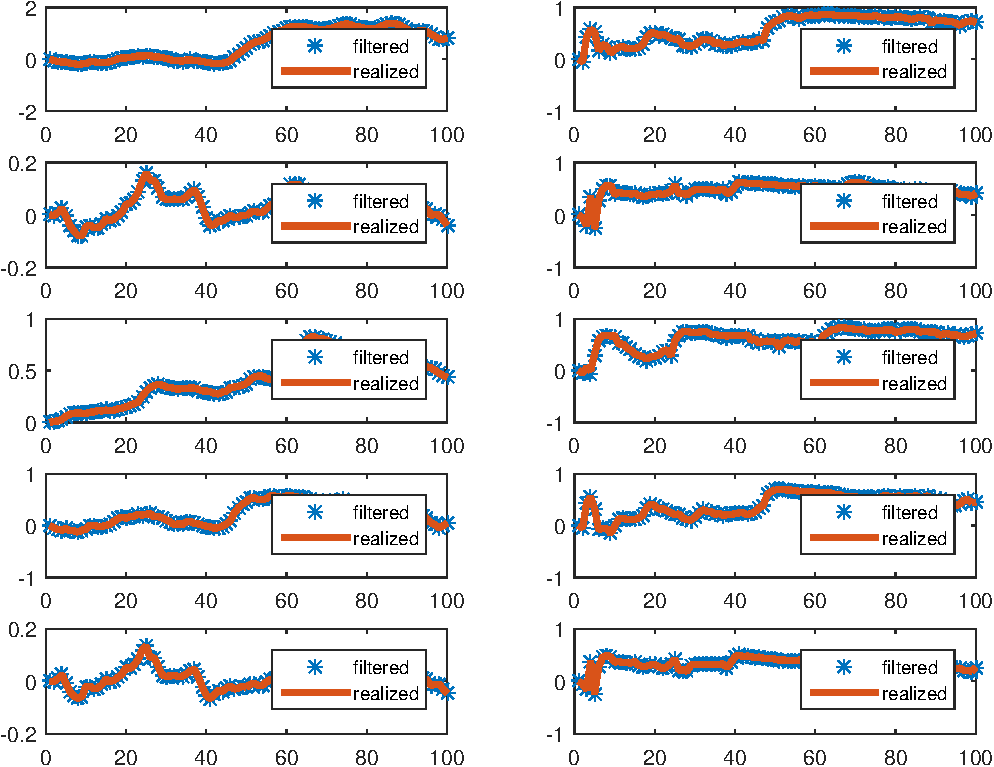
\includegraphics[scale=0.45]{MC_correctInit_beliefs.pdf} 
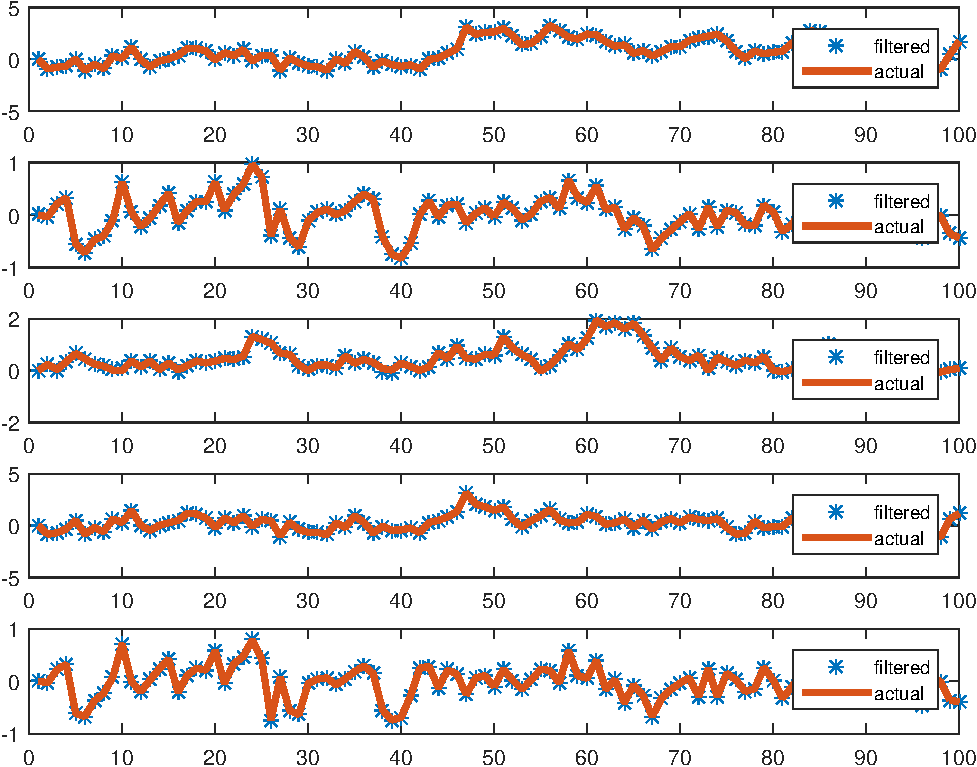
\includegraphics[scale=0.45]{MC_correctInit_states.pdf} \\
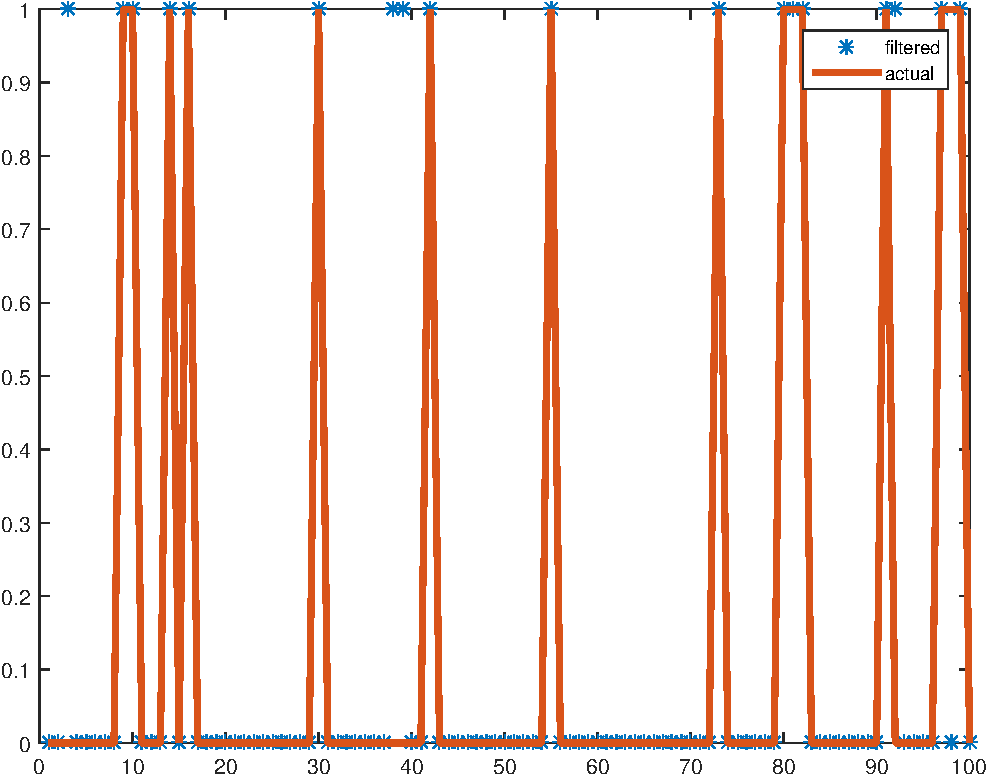
\includegraphics[scale=0.9]{MC_correctInit_stateProbabilities.pdf}\\
\end{figure}



\begin{figure}[H]
\small{\textbf{Plots from a typical simulation with randomized  initial states \& beliefs:}}\\

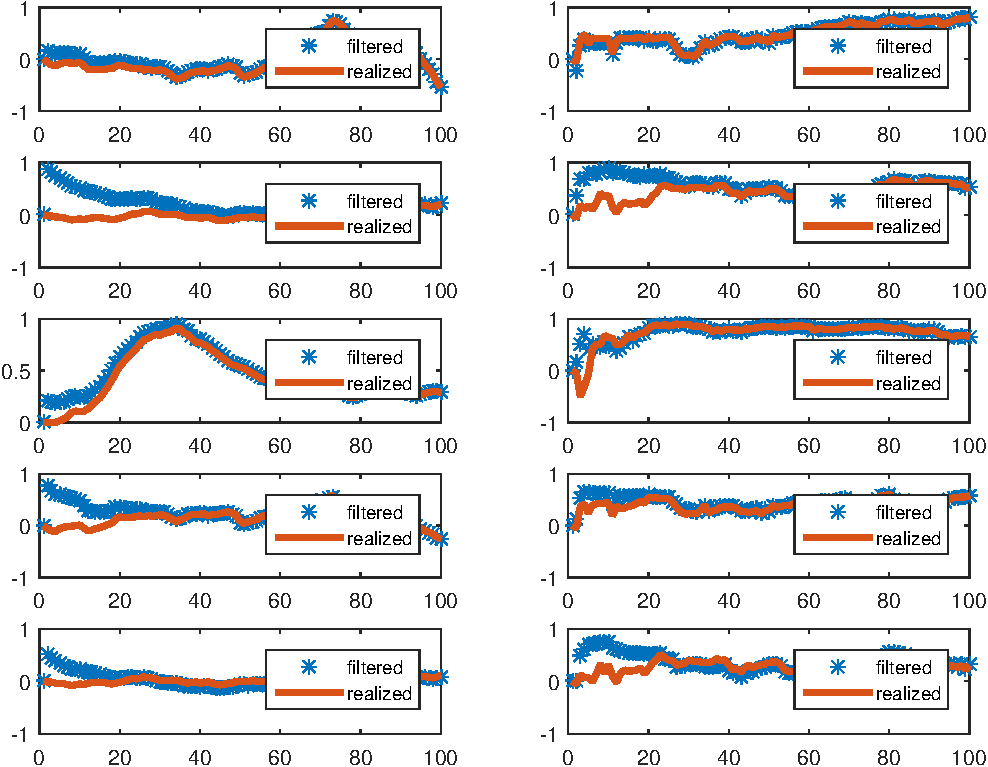
\includegraphics[scale=0.45]{MC_randomInit_beliefs.pdf} 
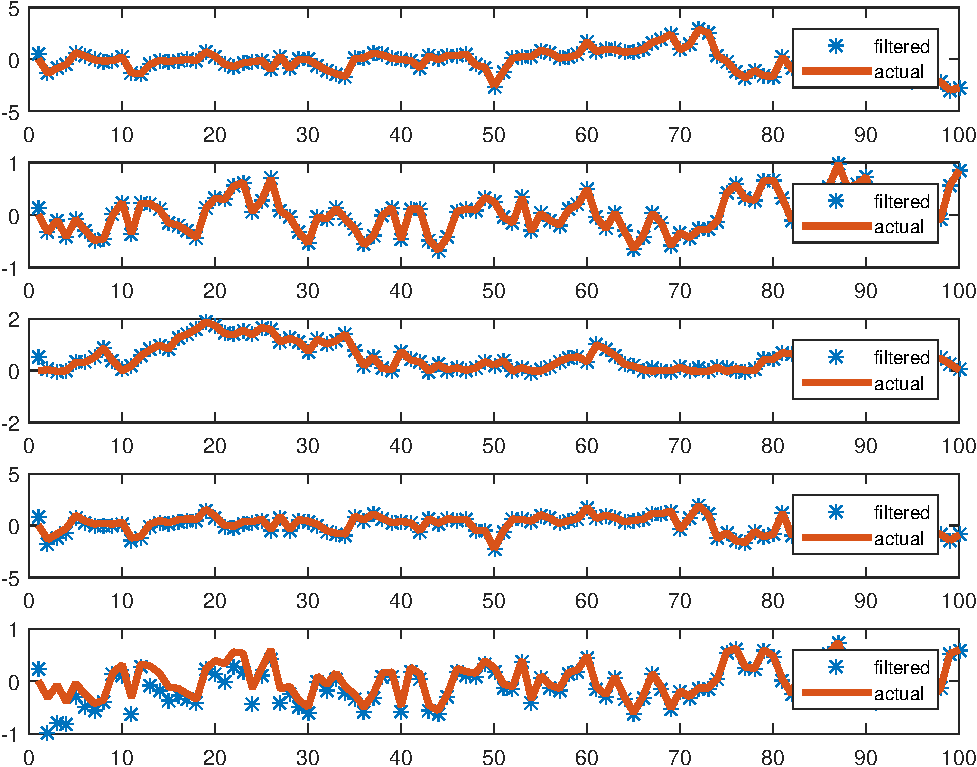
\includegraphics[scale=0.45]{MC_randomInit_states.pdf} \\
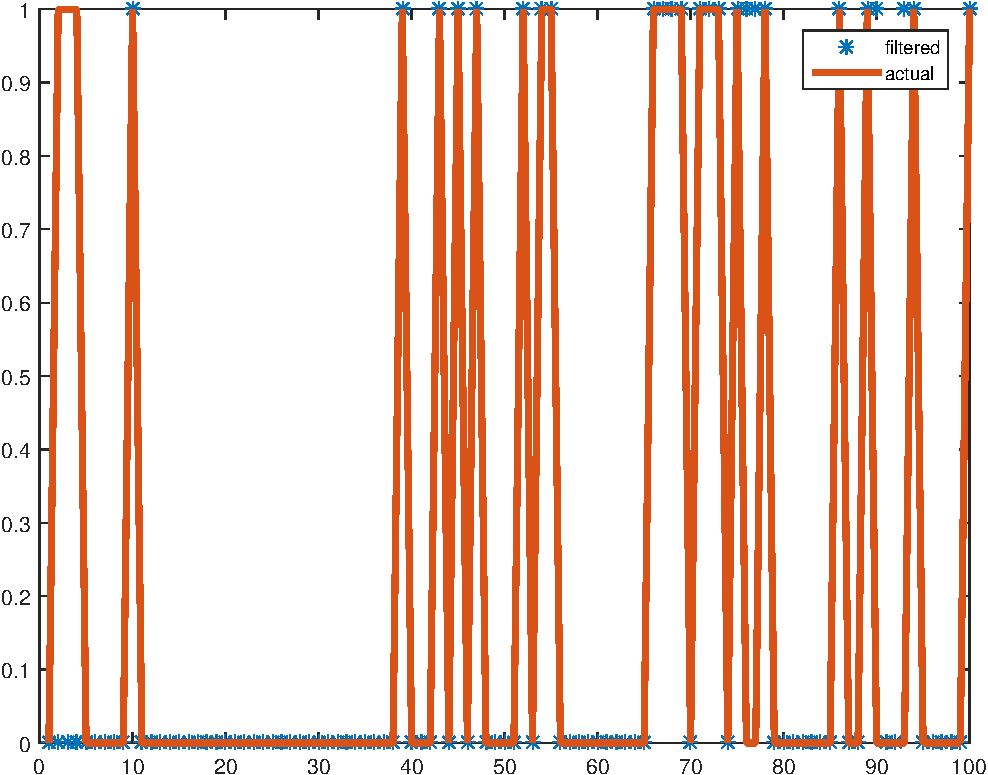
\includegraphics[scale=0.9]{MC_randomInit_stateProbabilities.pdf}\\

\end{figure}
\newpage

\textbf{\underline{Filtering with real data: ($1966:I-2016:IV$ U.S)}}\\

\begin{figure}[H]

{Decreasing gain learning:}  \\


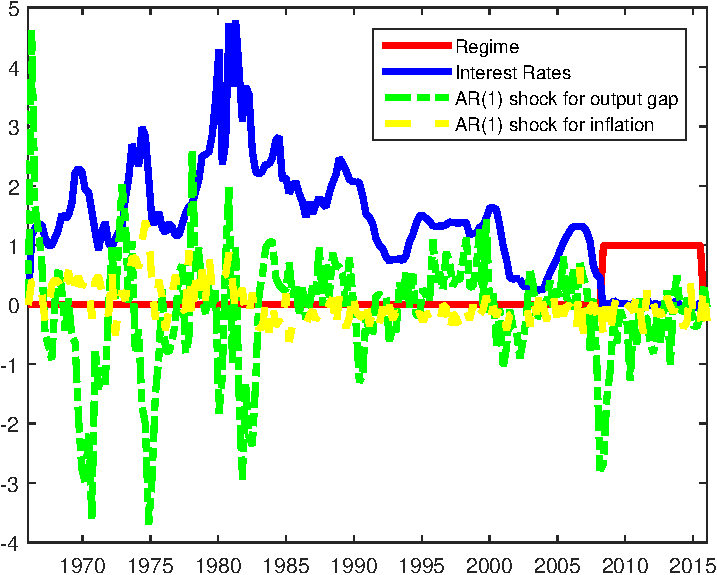
\includegraphics[]{NKPC_filteredRegimes_DGL.pdf}\\
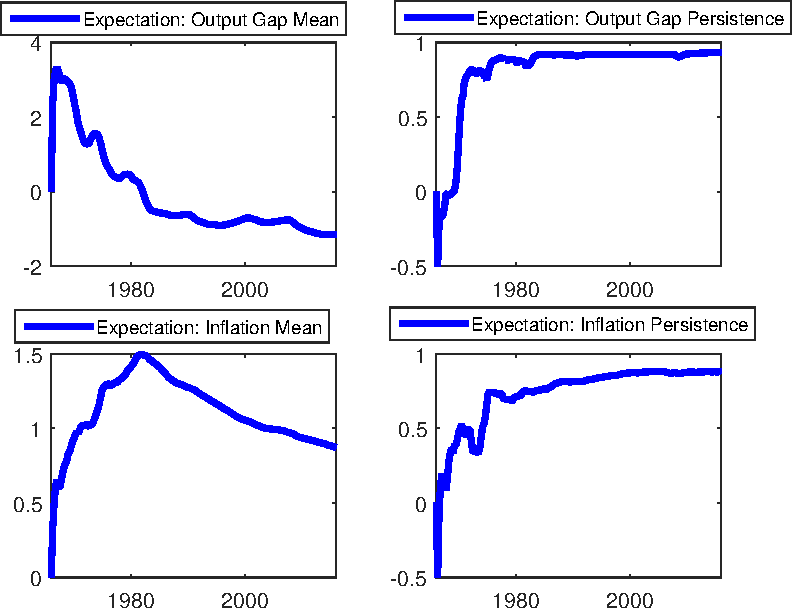
\includegraphics[]{NKPC_filteredBeliefs_DGL.pdf}\\
\end{figure}

\newpage

\begin{figure}[H]
	{Constant gain learning $ =0.05$:} \\


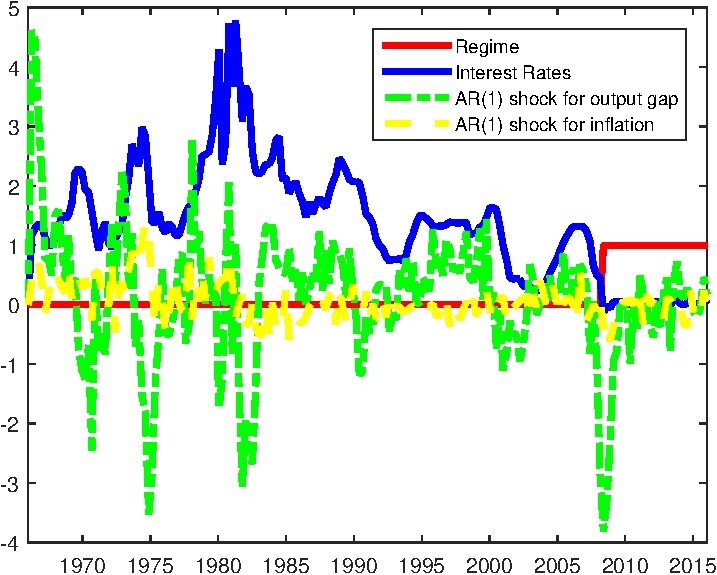
\includegraphics[]{NKPC_filteredRegimes_CGL.pdf}\\
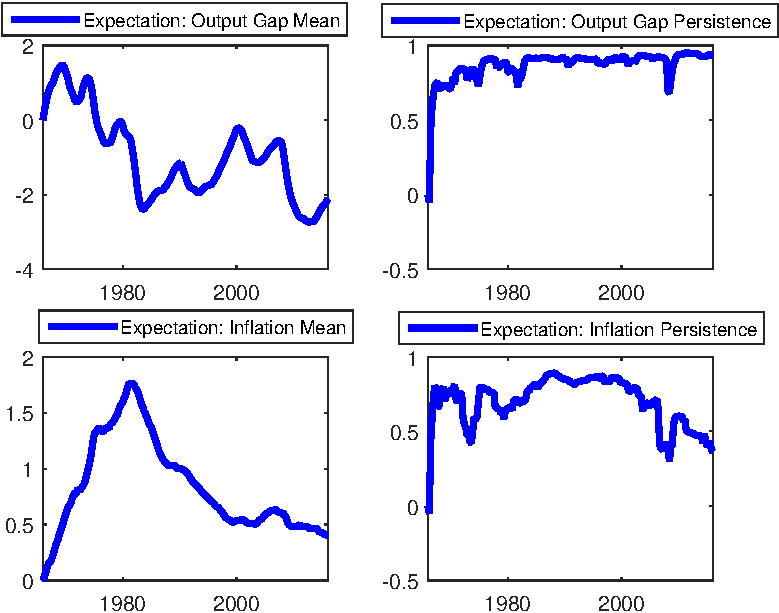
\includegraphics[]{NKPC_filteredBeliefs_CGL.pdf}\\
\end{figure}


\newpage



\begin{figure}
\textbf{\underline{Simulations of the Normal and \& ZLB Regimes:}} \\


{Normal Regime is E-stable:} \\

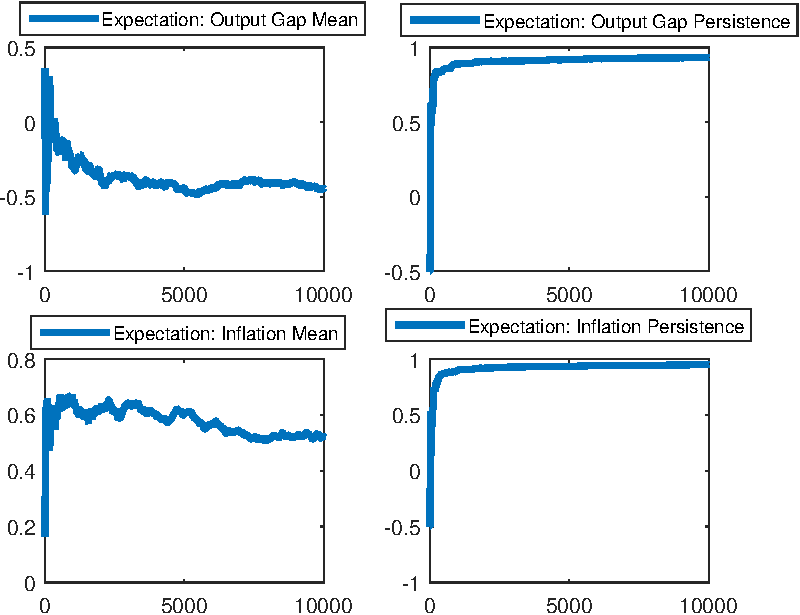
\includegraphics[scale=1]{simulation_normalRegime.pdf} \\

{ZLB Regime is not E-stable: } \\

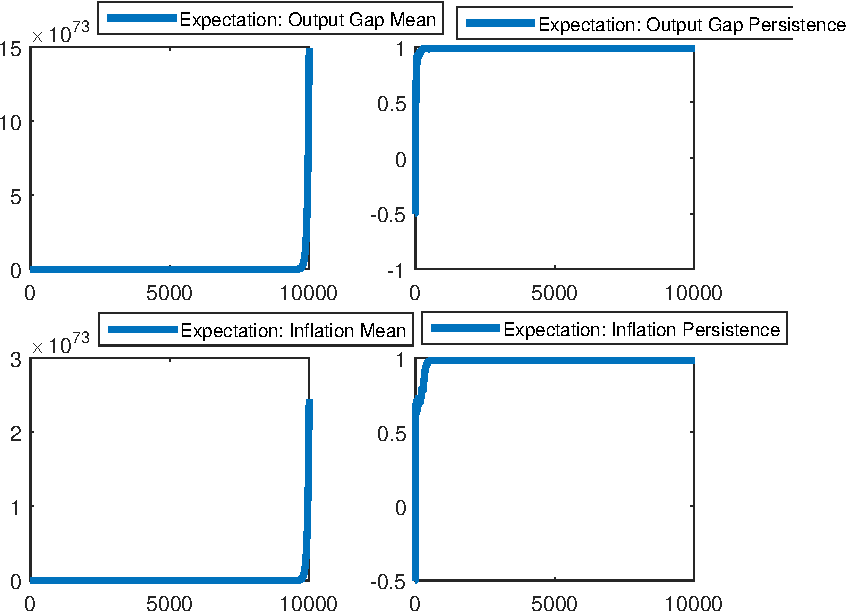
\includegraphics[scale=1]{simulation_zlbRegime.pdf}\\
\end{figure}




\subsection*{Markov Switching Filter with two lags}

\begin{figure}[H]
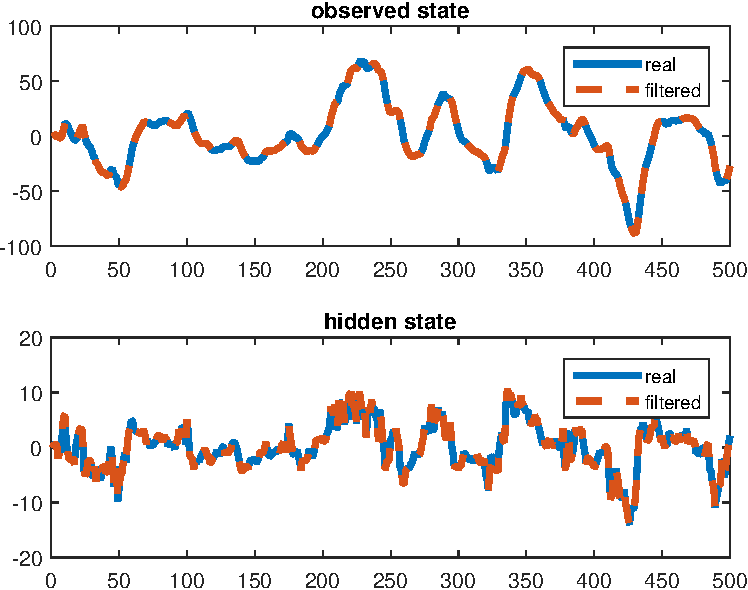
\includegraphics[]{MC_MS_small_states.pdf}\\

\end{figure}


\begin{figure}[H]
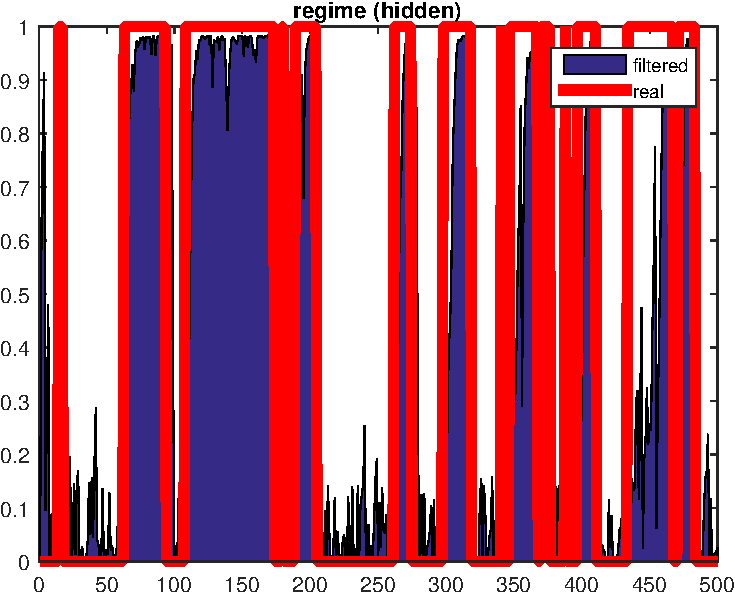
\includegraphics[scale=0.5]{MC_MS_small_regime1.pdf}
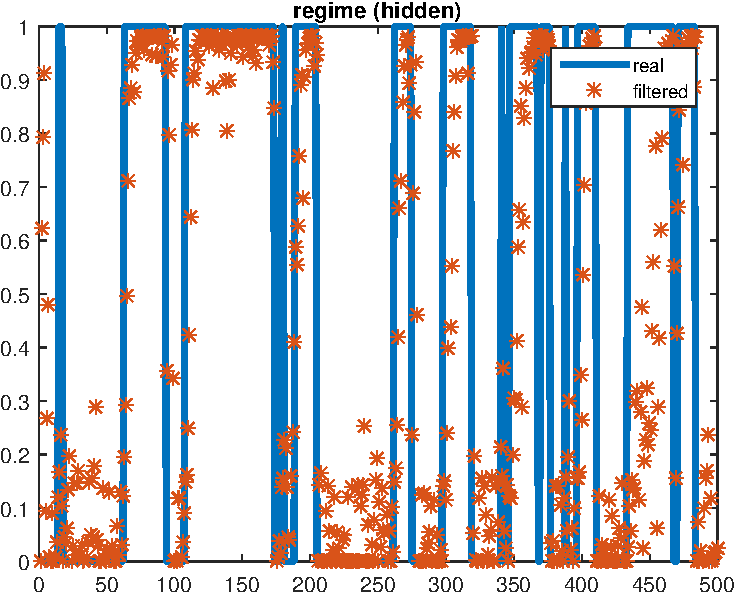
\includegraphics[scale=0.5]{MC_MS_small_regime2.pdf}\\

\end{figure}

\newpage

\end{comment}

\subsection*{Example 1:Fisherian Model of Inflation Determination}

$$
\begin{cases}
i_t = E_t \pi_{t+1} + r_t \\
r_t = \rho r_{t-1} + v_t \\
i_t = \alpha(s_t) \pi_t \\
\end{cases}
$$

where $ r_t $ is the exogenous AR(1) ex-ante real interest rate, $ i_t $ is the nominal interest rate and $\pi_t $ is inflation. Monetary policy follows a simple rule by adjusting nominal interest rate to inflation and changes stochastically between two regimes, with $s_t = \{1,2 \} $ and transition matrix:

$$
Q=\begin{pmatrix}
p_{11} & 1-p_{11} \\
1-p_{22} & p_{22} \\
\end{pmatrix}
$$

We can re-write the model in terms of inflation as follows: \\

$$
\begin{cases}
\pi_t = \frac{1}{\alpha(s_t)}(E_t \pi_{t+1} + r_t) \\
r_t = \rho r_{t-1} + v_t \\
\end{cases}
$$

When expectations are regime=dependent, the MSV-solution is of the form: $ \pi_{i,t} = \beta_i r_t $ (Davig \& Leeper, 2005). In this case, the model will be determinate as long as :\\

$$ (1-\alpha_2) p_{11} +(1-\alpha_1) p_{22} + \alpha_1 \alpha_2 > 1 $$. 

This is known as the long-run Taylor principle.\\
 

In this paper, we deviate from previous literature by assuming a regime-independent PLM of the form: \\

$$
\pi_t = a r_t  \Rightarrow E_t \pi_{t+1} = \beta E_t r_{t+1} = a \rho r_t 
$$

The implied ALM is then given by: \\

$$
\begin{cases}
\pi_t = \frac{1}{\alpha(s_t)} (\beta \rho + 1) r_t \\
r_t= \rho r_{t-1} + v_t 
\end{cases}
$$ 

Since the assumed PLM does not nest the regime-specific MSV solution, it can never converge to the underlying Rational Expectations Equilibrium. However, there is a non-rational equilibrium associated with the above PLM; this is commonly known as a Restricted Perceptions Equilibrium (RPE) in the adaptive learning literature. The value of $\beta$ corresponding to this RPE is pinned down by unconditional moment restrictions. Accordingly, $\frac{E [\pi_t r_t]}{E[r_t r_t]} $ should match in implied ALM and PLM\footnote{In principle, we can use any other moment restrictions to pin down the value of $\beta$. We use this moment since it yields the least complicated expressions.}. \\

-In PLM, we have: $\frac{E [\pi_t r_t]}{E[r_t r_t]} =\beta $.\\

-In implied ALM, we have: $\frac{ E[\pi_t r_t]}{E[r_t r_t]} = E[ \frac{1}{\alpha(s_t)} \beta \rho + \frac{1}{\alpha(s_t)}]$.

The unconditional moment in implied ALM above requires the ergodic distribution of the Markov chain: $ \pi' Q = \pi $. \\

We get $ \pi = [ \frac{1-p_{22}}{2-p_{11}- p_{22}}, \frac{1-p_{11}}{2-p_{11}-p_{22}}] $. \\

This yields $ \beta = \frac{1}{\sum_i \pi_i \alpha_i  -\rho } $, and the solution reduces to: \\

$$ \pi_t = \frac{1}{\sum_i \pi_i \alpha_i  -\rho} r_t $$

\underline{E-stability} \\

The mapping from agents' PLM to the implied ALM is defined as the T-map. In our example, this mapping is given by: \\

$$ T: a \rightarrow \frac{\beta \rho + 1 }{\sum_i \pi_i \alpha_i} $$

The T-map is locally stable if its Jacobian matrix has eigenvalues with real parts less than one. When this local stability condition is satisfied, the equilibrium is said to be E-stable (Evans \& Honkapohja, 2001). In our example, the Jacobian is given by: \\

$$ \frac{DT(\beta)}{D(\beta)} = \frac{\rho}{\sum_i \pi_i \alpha_i} $$. 

Hence the equilibrium is E-stable if the largest eigenvalue has real part less than one, i.e. $\frac{\rho}{\sum_i \pi_i \alpha_i} < 1 $. \\

With two regimes and $\alpha_2 = 0 $, the E-stability condition reduces to : \\

$$ \alpha_1 > \frac{\rho}{\pi_1} $$


In general, in order to satisfy E-stability, we need a stronger monetary policy rule $\alpha_1 $ whenever: \\

-The average time spent in regime 1 ($\pi_1 $) decreases, \\
-The average time spent in regime 2 ($\pi_2 $) increases, \\
-The monetary policy rule in regime 2 ($\alpha_2 $) weakens.\\

Intuitively, this result is a simple extension of the long-run Taylor principle of David \& Leeper (2005). (Maybe we shall call this the long-run E-stability principle??) \\


\newpage

\underline{Simulations with least squares updating:}\\

$$
\begin{cases}
R_t = R_{t-1} + \gamma (r_t^2 - R_{t-1} ) \\
\beta_t = \beta_{t-1} + \gamma R_t^{-1} r_t (\pi_t - \beta_{t-1} r_t) 
\end{cases}
$$

Parameters: $\rho = 0.9, p_{11}=0.95, p_{22}= 0.95, \eta_{\sigma} = 0.1, \gamma=0.001 $, where $\gamma $ denotes the gain parameter. \\

Case (i) Both underlying regimes are E-stable: $ \alpha_1 = 2, \alpha_2 = 1.5 $. \\
In this case the coefficient fluctuates between the regime-specific equilibrium values depending on which regime is realized. On average, it fluctuates around the long-run (or unconditional) equilibrium value. \\

Case (ii) One E-stable and one E-unstable : $ \alpha_1 = 2, \alpha_2 = 0.5 $. \\
In this case the coefficient will show explosive-like dynamics (does this relate to escape dynamics?) when the realized regime is E-unstable, but will revert back to the long-run equilibrium when the system switches back to the E-stable regime. 

\begin{figure}[H]
\caption{Left panel: Case (i) with two E-stable regimes. Right panel: Case (ii) with one E-stable and one E-unstable regime. }
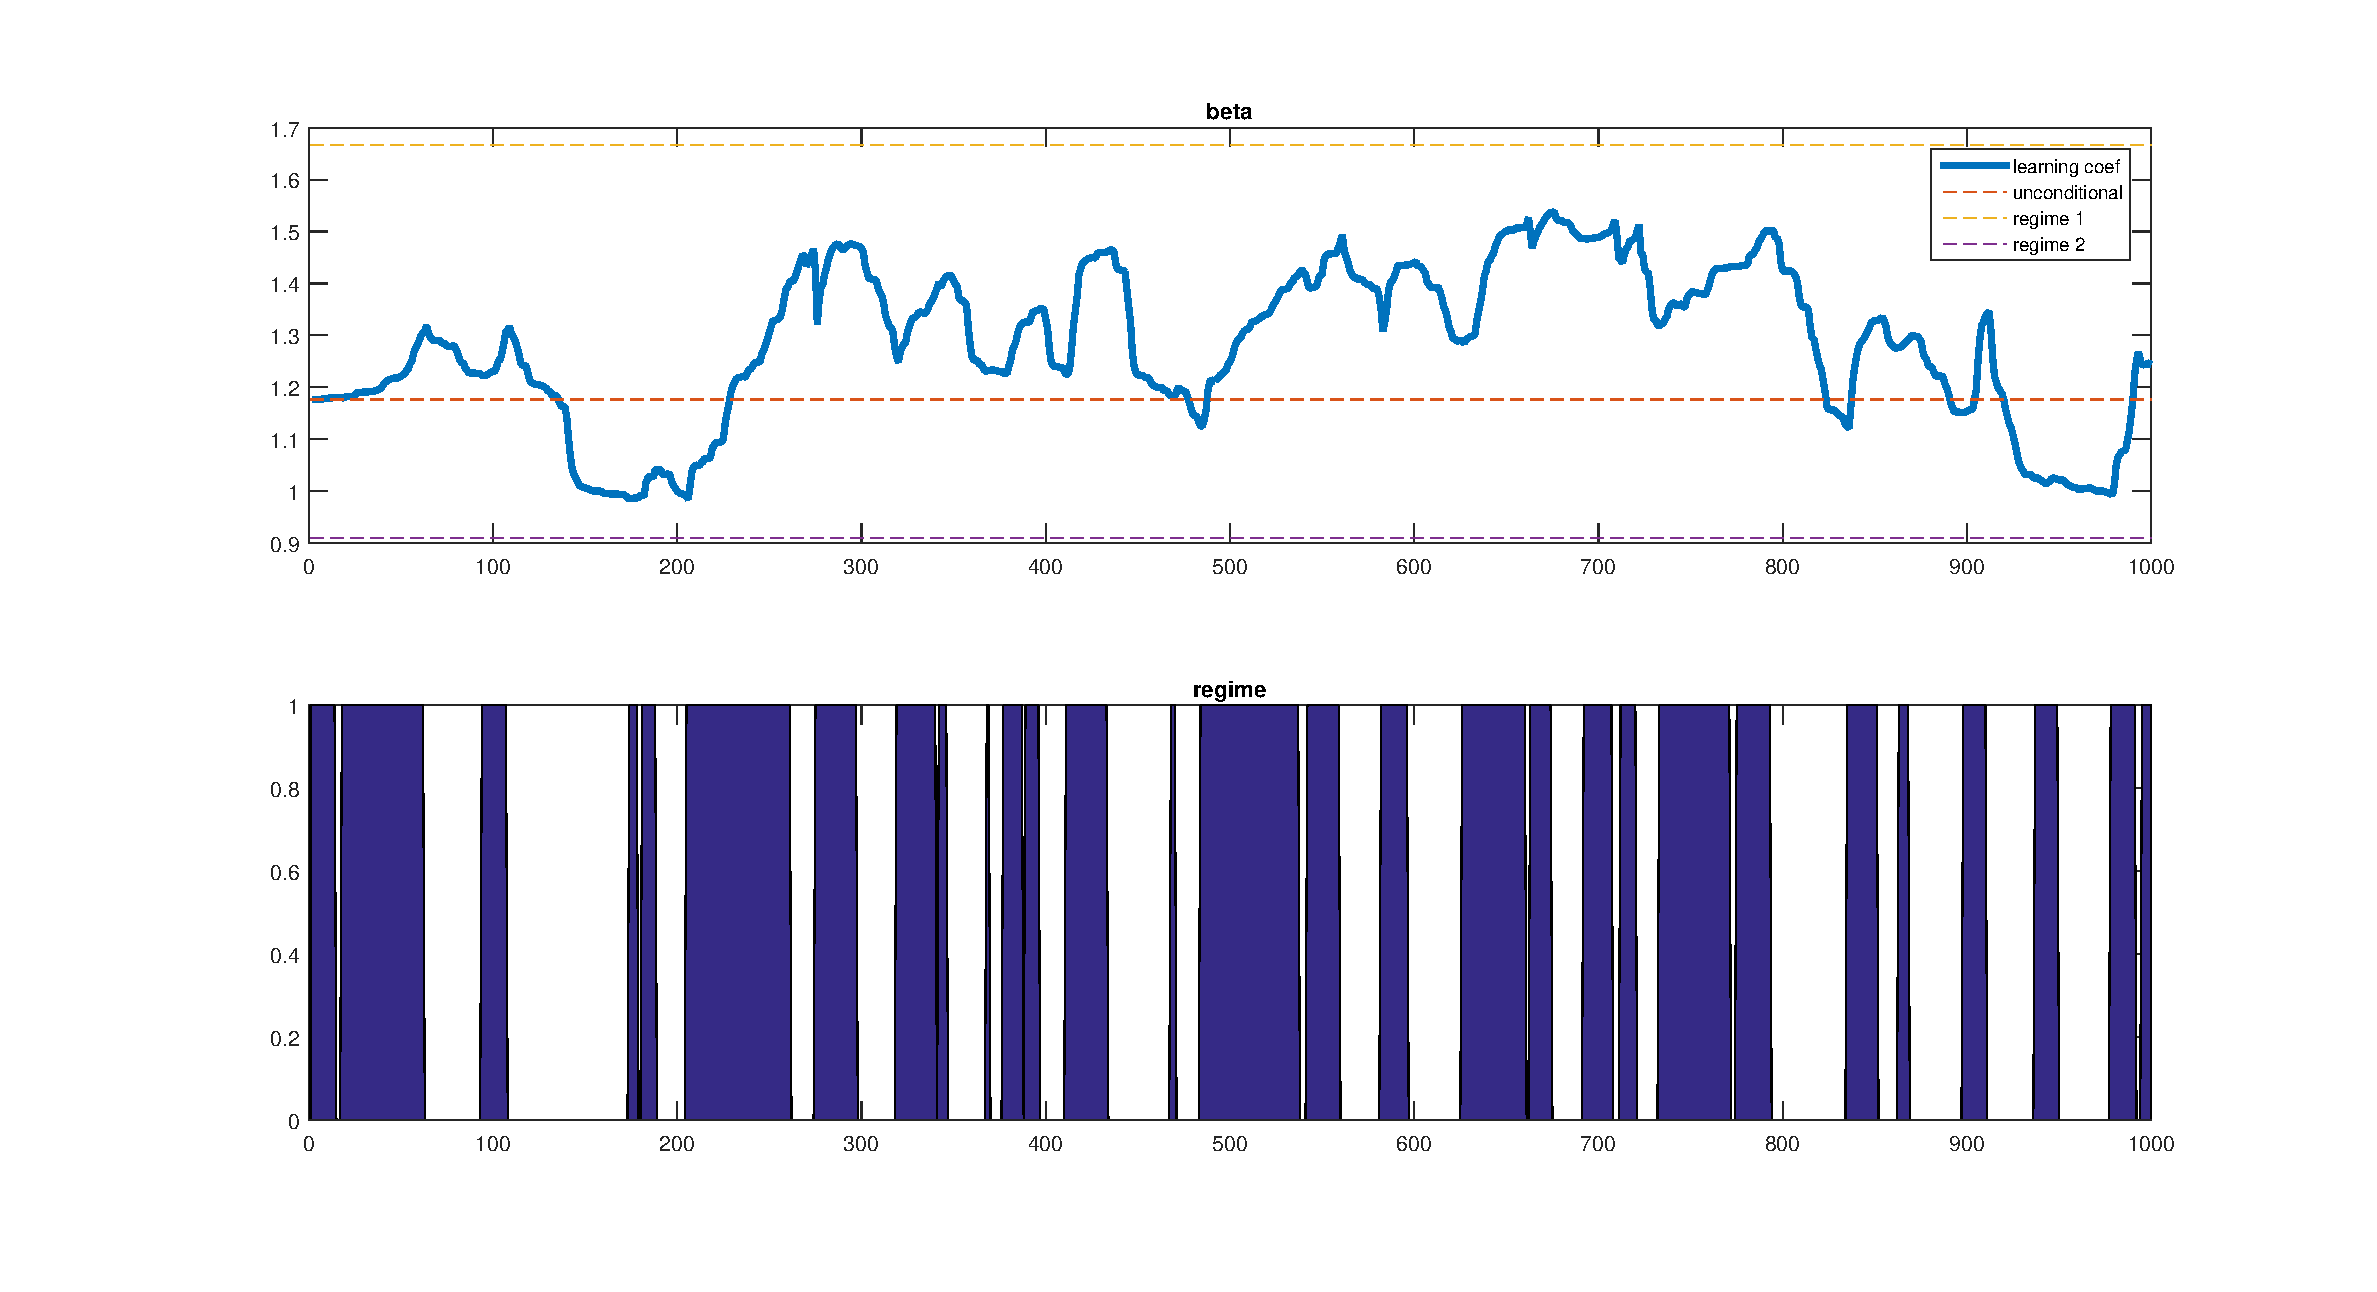
\includegraphics[scale=0.6]{fisher_simulation1_learningCoef.pdf} 
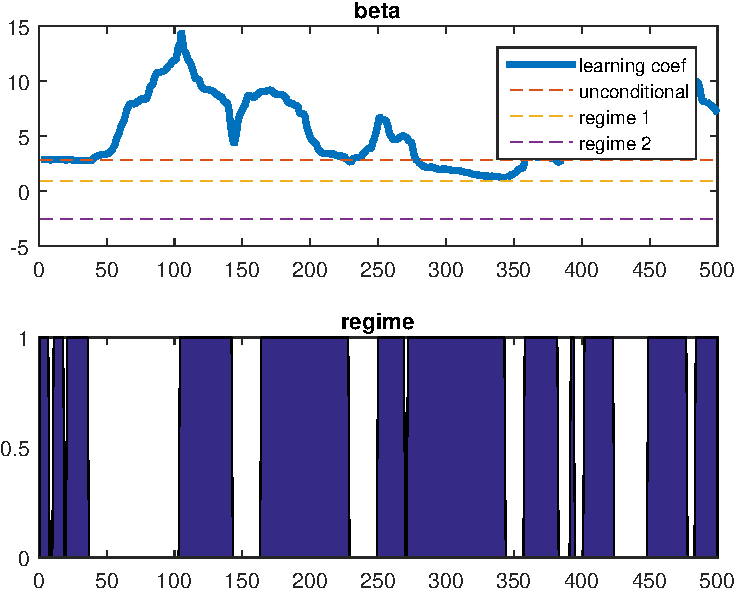
\includegraphics[scale=0.6]{fisher_simulation2_learningCoef.pdf} \\
%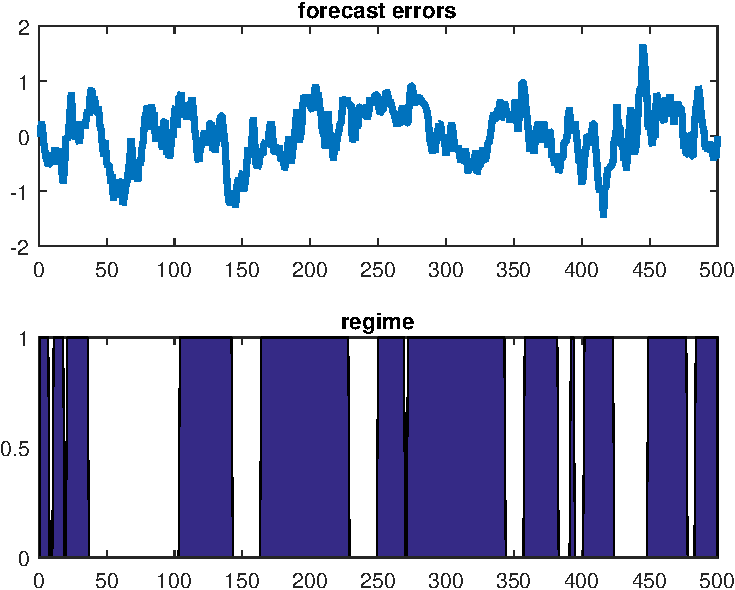
\includegraphics[scale=0.6]{fisher_simulation1_FE.pdf} \\
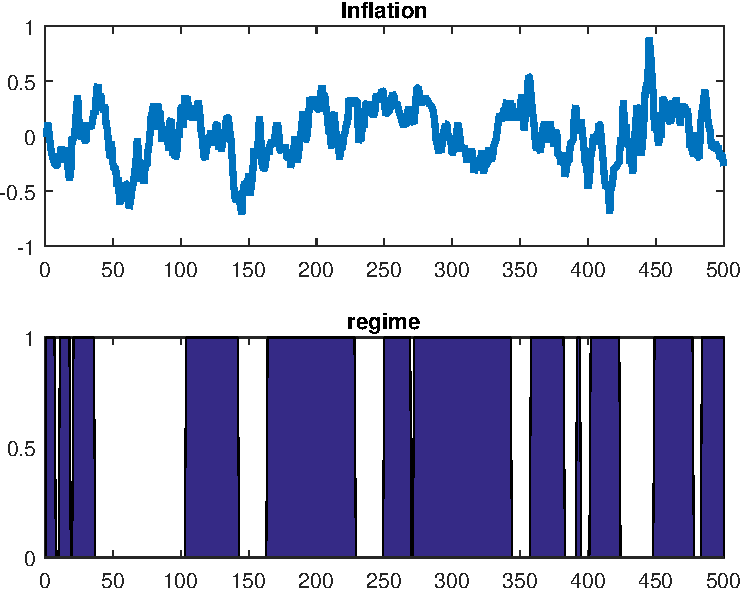
\includegraphics[scale=0.6]{fisher_simulation1_pinf.pdf} 
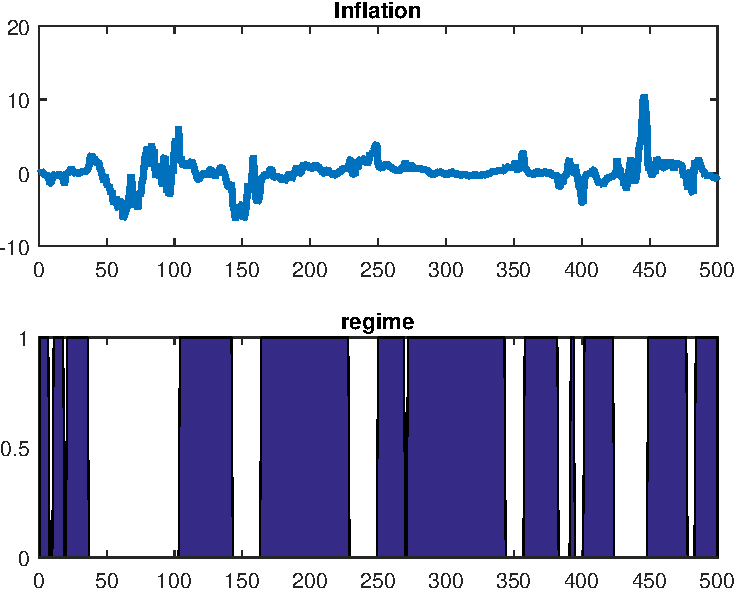
\includegraphics[scale=0.6]{fisher_simulation2_pinf.pdf} \\
\end{figure}



\newpage

\subsection*{Example 2: 3-equation model without lagged endogenous variables} 

Now consider the baseline 3-equation NKPC model along the lines of Woodford (2003), where the interest rate is subject to the ZLB constraint. 
$$
\begin{cases} 
x_t = E_t x_{t+1}  -\frac{1}{\tau}(r_t - E_t \pi_{t+1})+ \epsilon_{x,t} \\
\pi_t = \beta E_t \pi_{t+1} + \kappa x_t + \epsilon_{\pi,t} \\
r_t = max\{ 0, \phi_x x_t + \phi_{\pi} \pi_t + \eta_{r,t}\} \\
\epsilon_{y,t} = \rho_y \epsilon_{y,t-1} + \eta_{y,t} \\ 
\epsilon_{\pi,t} = \rho_{\pi} \epsilon_{\pi,t-1} + \eta_{\pi,t} \\
\end{cases} 
$$

We can re-cast the interest rate rule above as a Markov process with two regimes, where: \\

$$
\begin{cases}
r_t (s_t=1) = \rho r_{t-1} +(1-\rho) (\phi_x x_t + \phi_{\pi} \pi_t) + \eta^{1}_{r,t}\} 
r_t (s_t=2) =\eta^{2}_{r,t}\} 
\end{cases}
$$

with the transition matrix same as in the first example. The presence of noise in the second regime is meant to capture the fact that, although interest rates are very close to zero in empirical data, they are never exactly equal to zero in the post-2007 period. The above model can then be re-written as follows: \\

$$
\begin{cases}
X_t = C(s_t) E_t X_{t+1} + D(s_t) \epsilon_t \\
\epsilon_t = \rho \epsilon_{t-1} + \eta_t \\
\end{cases}
$$

The regime-independent PLM and one-step ahead expectations are given by: \\

 $ X_t = d \epsilon_t \Rightarrow E_t X_{t+1} = d \rho \epsilon_t $.\\

which yields the implied ALM:\\

$$
\begin{cases}
X_t = C(s_t) d \rho \epsilon_t+ D(s_t) \epsilon_t \\
\epsilon_t = \rho \epsilon_{t-1} + \eta_t \\
\end{cases}
$$

Imposing the following moment restriction for consistency yields: \\

$ \frac{ E[X_t \epsilon_t]}{E[\epsilon_t \epsilon_t]}= d  $  in PLM; this should be equal the the corresponding unconditional moment in ALM. Solving yields: \\

$ d = \sum_i C_i \pi_i d \rho + \sum_i \pi_i D_i $. \\

Hence 
$$ vec(d) = (I-\rho \otimes (\sum_i C_i))^{-1} vec(\sum_i \pi_i D_i ) $$

In this case the T-map is given by : \\

$$ T : d \rightarrow \sum_i \pi_i C_i d \rho + \sum_i D_i \pi_i $$

with Jacobian matrix  $ \frac{DT }{D d} = vec^{-1}(\rho' \otimes \sum_i \pi_i C_i) $. If all eigenvalues of this expression have real parts less than one, then the equilibrium is locally stable under least squares learning. 

\newpage 

\textbf{Monte Carlo Simulations: } \\

Parameters: $\phi_y =0.5, \phi_{\pi}=1.5, \kappa=0.01, \beta=0.99, \sigma_y = 0.7, \sigma_{\pi} =0.3, \sigma^{I}_r =0.3, \sigma^{II}_r=0.01,\rho_y =0.5, \rho_{\pi}=0.5 , p_{11} = 0.99, p_{22} = 0.9, \gamma = 0.01$. In each case, we simulate the model 500 times with a length of 10000 periods. We then collect the final values of learning coefficients in PLM. \\


\begin{figure}[H]
\caption{Case (i): Least squares updating in NKPC without regime-switching (i.e. this is the standard adaptive learning case). First row: intercept terms (should converge to zero). Second \& third rows: lagged inflation and output gap (should converge to zero). Fourth \& fifth rows: coefficients on output gap and inflation shocks (should be non-zero). The red lines correspond to the underlying REE.  }

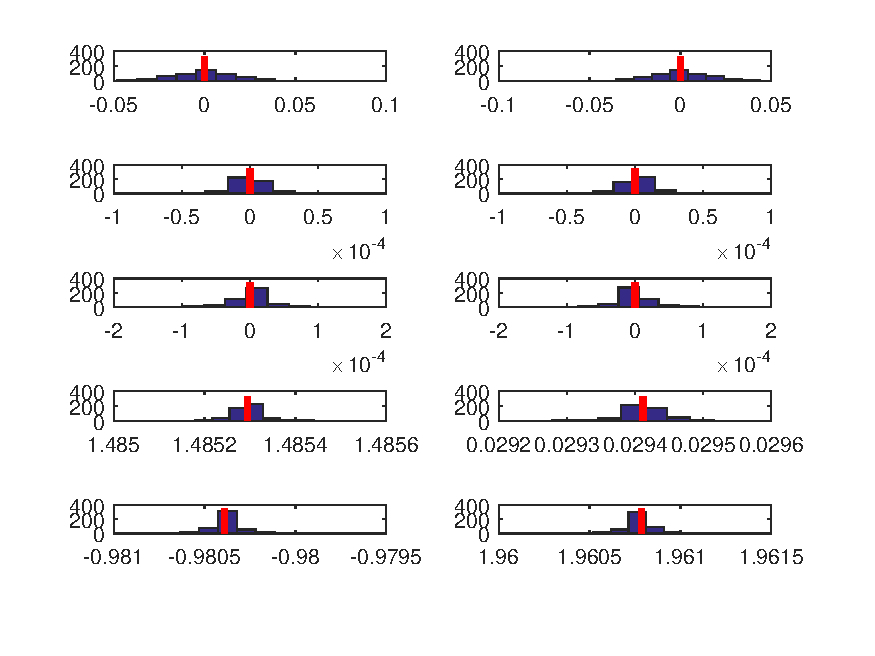
\includegraphics[scale=1.2]{MC_MSV_withoutLags.pdf}\\
\end{figure}

\newpage



\begin{figure}[H]
\caption{ Case (ii): Least squares updating NKPC with two regimes as outlined above.   First row: Intercept terms (should converge to zero). Second \& third rows: coefficients on output gap and inflation shocks (these should be non-zero). The coefficients on shocks should converge to the RPE as given above; these values are again denoted by the red lines. For these simulations, we do not include the lagged inflation and output gap in PLM (If they are included, they should converge to zeros similar to the case above). } 

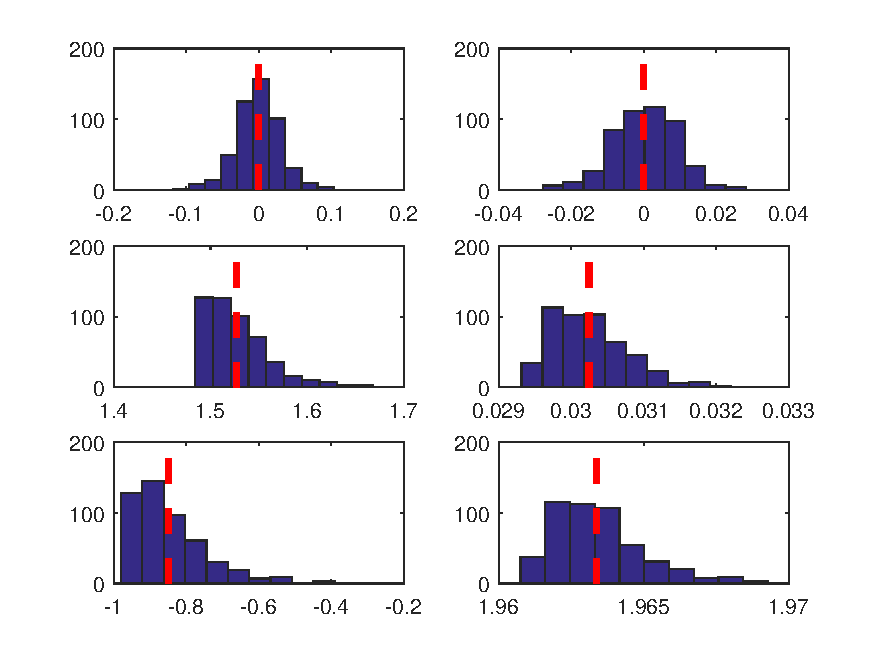
\includegraphics[scale=0.6]{MC_MS_MSV_withoutLags.pdf}\\
\end{figure}



\begin{figure}[H]
\caption{Typical simulation from Markov-switching exercise above:} 
\textbf{Intercept terms:} \\
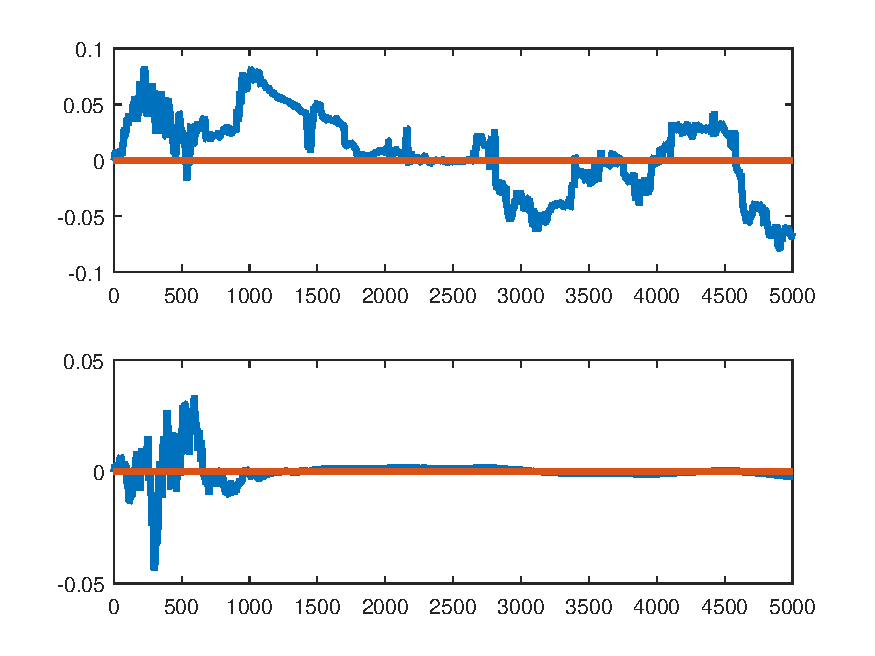
\includegraphics[scale=0.4]{MS_simulation_alphas.pdf}\\
\textbf{Shock coefficient terms: } \\
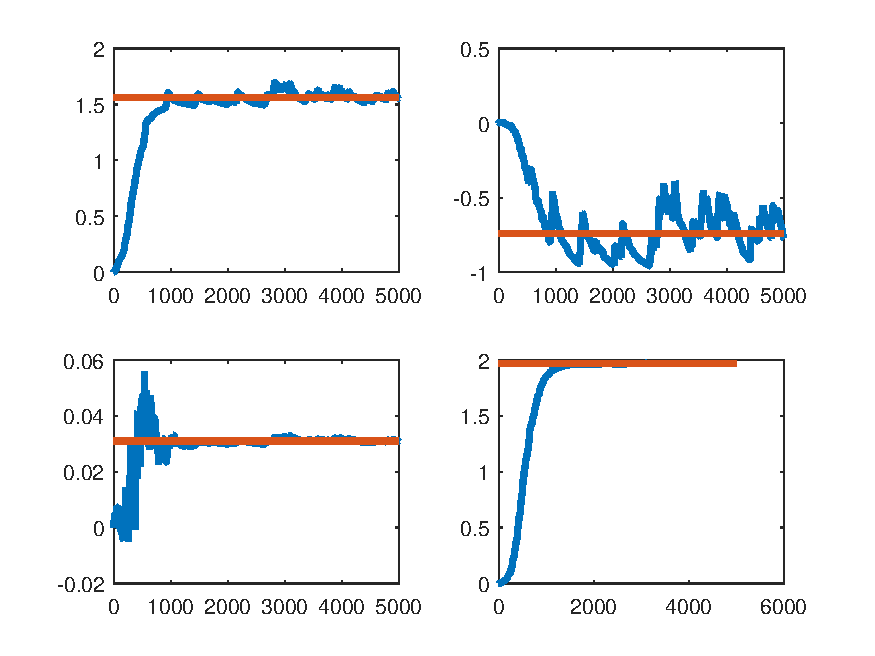
\includegraphics[scale=0.4]{MS_simulation_shockCoef.pdf}\\
\end{figure}

\subsection*{General Case I : MSV learning} 

In the above examples considered, lagged state variables do not enter into the model. In these cases, the underlying RPE takes a simple form that can be computed analytically. However, in empirically relevant models, lagged state variables typically enter into the model equation (via habit formation, price / wage indexation, interest rate smoothing, etc.). In this section we consider MSV-learning where the lagged state variables are included in the model. Consider the model of the form: \\

$$
\begin{cases}
X_t = A(s_t) + B(s_t) X_{t-1} + C(s_t) E_t X_{t+1} + D(s_t) \epsilon_t \\
\epsilon_t = \rho \epsilon_{t-1} + \eta_t 
\end{cases}
$$

PLM takes the form of MSV solution but is regime-independent, which is given by (along with the one-step ahead expectations) : \\

$$
\begin{cases}
X_t = a + b X_{t-1} + d \epsilon_t \\
E_t X_{t+1} = (a+ba) + b^2 X_{t-1} + (bd + d\rho) \epsilon_t 
\end{cases}
$$
which yields the implied ALM: \\

$$
X_t = ( A(s_t) + C(s_t) (a+ba) ) + (C(s_t) b^2 + B(s_t))X_{t-1} + ( C(s_t) (bd +d \rho ) + D(s_t) ) \epsilon_t 
$$

For the remainder, we use the notation $\tilde{m} = \sum_i \pi_i m_i $ for the weighted average of any matrices $m_i $. Imposing the moment restrictions in this case yields: \\

$$
\begin{cases}
a = E[ A(s_t) + C(s_t)  (a+ba)]= \tilde{A} + \tilde{C} (a+ba) \\
b=E[C(s_t) b^2 + B(s_t)]=\tilde{C} b^2 + \tilde{B} \\
d = E[C(s_t) (bd+d \rho) + D(s_t)] = \tilde{C} (bd + d \rho ) + \tilde{D} 
\end{cases}
$$

In the above expression, $ a $ and $ d $ can be obtained for a given b. However, the second equation is quadratic in b. With $n $ endogenous variables, this can in principle have up to $ {2n}\choose{n} $ solutions in $b$ (Check this!). \\

In this case, the T-map is given by: \\

$$
\begin{pmatrix} a \\ b \\ d \end{pmatrix} \rightarrow \begin{pmatrix} \tilde{A} + \tilde{C} (a+ba) \\ \tilde{C} b^2 + \tilde{B} \\  \tilde{C} (bd+d \rho) + \tilde{D} \end{pmatrix}
$$

Denoting $\theta = (a,b,d)' $, the associated Jacobian is : \\

$$ \frac{ D T } { D\theta }  = \begin{bmatrix} \tilde{C} + \tilde{C} b & vec_{n,n}^{-1} (a' \otimes \tilde{C}) & 0 \\
0 & 2 \tilde{C} b & 0 \\
0 & vec_{n,n}^{-1}(d' \otimes \tilde{C} ) & \tilde{C} b + vec_{n,n}^{-1} (\rho' \otimes \tilde{C} ) \end{bmatrix} $$

where $ vec_{n,n}^{-1} $ denotes the matricization of a vector to an $(n,n) $ matrix. \\

The eigenvalues of the Jacobian above are given by the terms on the diagonal. Hence the underlying RPE is E-stable if these eigenvalues have real parts less than one. \\

(these eigenvalues include the $ b $ term itself, i.e. $b $ will converge to something if $b $ satisfies a certain condition. Does this make sense? Cars' paper had something similar and the referees didn't like it, is it the same thing? ) \\

Although we cannot obtain an explicit expression for the underlying equilibrium, we can still simulate the model and check whether the coefficients converge somewhere. The figure below provides the same exercise as in the previous section, where we add an interest rate smoothing coefficient of $0.9$ to the interest rate rule in the first regime.



\begin{figure}[H]
\caption{Distributions from 500 simulations of length 10000 for the two-regime NKPC. First row: intercept terms (should converge to zero). Second and third rows: lagged inflation and output gap coefficients (should converge to zero as they do not belong in the MSV-rule). Fourth row: Lagged interest rate: should converge to non-zero values given non-zero interest rate smoothing. Fifth and sixth rows: Coefficients on output gap and inflation shocks: should converge to non-zero values. Overall, we observe similar distributions compared to the switching (and also non-switching) case of previous section, indicating convergence towards an equilibrium. }
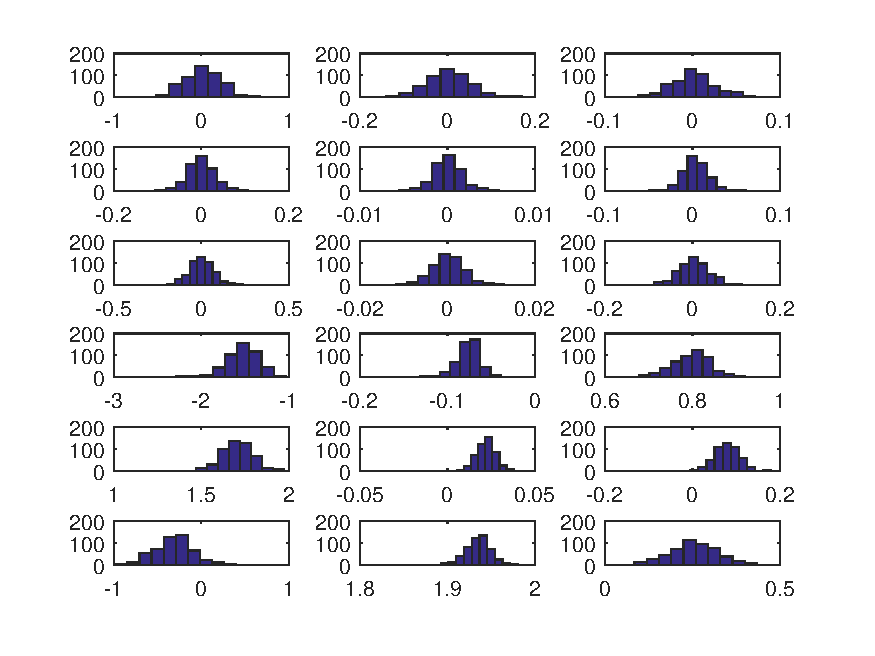
\includegraphics[scale=1]{MC_MS_MSV_withLags.pdf}\\
\end{figure}


\newpage


\subsection*{General Case II: VAR(1) learning} 

So far we considered MSV-type of learning, where the only source of misspecification in PLM comes from the fact that expectations are not regime-specific. In general, however, we can consider any type of misspecification in the PLM and there may exist an E-stable RPE associated with the given PLM. In this section, we extend our analysis to VAR(1)-type rules with unobserved shocks. 
Accordingly, consider again models of the form:

$$
\begin{cases}
X_t = A(s_t) + B(s_t) X_{t-1} + C(s_t) E_t X_{t+1} + D(s_t) \epsilon_t \\
\epsilon_t = \rho \epsilon_{t-1} + \eta_t 
\end{cases}
$$

Since shocks are assumed to be unobserved, we can stack up the endogenous variables $X_t $ and exogenous shocks $\epsilon_t $ into a vector $ S_t = [X_t' \hspace{3 mm}\epsilon_t']' $ to obtain models of the form: \\

$$
S_t = \gamma_0 (s_t) + \gamma_1 (s_t) S_{t-1} + \gamma_2(s_t) E_t S_{t+1}  + \gamma_3 (s_t) \eta_t
$$

Assume the PLM, and the one-step ahead expectations take the form: \\

$$
\begin{cases}
S_t = a + b S_{t-1} + u_t \\
E_t S_{t+1} = (a+ba)+ b^2 S_{t-1} 
\end{cases}
$$

Implied ALM is given by: \\

$$ 
S_t = (\gamma_0 (s_t) + \gamma_2 (s_t) (a+ba))+ (\gamma_1 (s_t) +\gamma_2 (s_t) b^2 )S_{t-1} + \gamma_3(s_t) \eta_t 
$$

In cases where the matrix $b $ does not exactly coincide with the functional form of the MSV solution, the consistency requirements do not simplify. \\

$ E [ S_t ] = (I-b)^{-1} a  $ in PLM.  \\

$ E [S_t] = ( I -  \tilde{\gamma_1} - \tilde{\gamma_2} b^2 )^{-1} (\tilde{\gamma_0} + \tilde{\gamma_2}(a+ba)  ) $ in ALM. \\

The vector $ a $ in the expression above can be solved for a given $ b $. Next we turn to the consistency requirement for the matrix $ b $. Note that in PLM, we have : \\

$ E [ \tilde{S_t} \tilde{S_t}']^{-1} E [ \tilde{S_t} \tilde{S_{t-1}}'] = b $, where $\tilde{S_t} = S_t - E[S_t]$. Hence we turn to computing these moments in ALM. Denoting by $\Gamma_0 $ and $\Gamma_1 $ the variance and autocovariance matrices respectively, the first two Yule-Walker equations of the ALM are given as : \\

$$
\begin{cases}
\Gamma_1 = \tilde{M}(b) \Gamma_0 \\
\Gamma_0 = \tilde{M}(b) \Gamma_0 \tilde{M}(b)' + \tilde{\gamma_3}\Sigma_{\eta} \tilde{\gamma_3}' 
\end{cases}
$$

where $\tilde{M}(b) = \tilde{\gamma_1} + \tilde{\gamma_2} b^2$. Solving the second expression above yields 
$$ vec(\Gamma_0) = (I- \tilde{M}(b) \otimes \tilde{M}(b))^{-1} (\tilde{\gamma_3} \otimes \tilde{\gamma_3}) vec(\Sigma_{\eta}) $$

Hence for each term $b(i,j) $, we have $ b(i,j) = \frac{vec(\Gamma_1)_{(j-1)N+j}}{vec(\Gamma_0)_{(j-1)N+j}} \Rightarrow b = \Gamma_1 \oslash \Gamma_0 $. \\

In the special case where $ b $ takes the form of the corresponding MSV matrix on lagged endogenous terms, the solution for $ b $ reduces to the quadratic equation $ b = \tilde{\gamma_1 } + \tilde{\gamma_2 } b^2 $ as in the previous case. \\

The T-map in this case is given by the following: \\

$$
T: \begin{pmatrix} a \\ b \end{pmatrix}  \rightarrow \begin{pmatrix} \tilde{\gamma_0} + \tilde{\gamma_2} (a+ba) \\ \tilde{\gamma_1} + \tilde{\gamma_2} b^2 \end{pmatrix} 
$$

Denoting $ \theta = (a,b) $ , the corresponding Jacobian is \\

$$
\frac{DT}{ D \theta} = \begin{bmatrix}  \tilde{\gamma_2 } (I+b) & vec^{-1}_{n,n} ( a' \otimes \tilde{\gamma_2}) \\ 0 & 2 b \tilde{\gamma_2}  \end{bmatrix} 
$$
Hence the corresponding RPE will be E-stable if the eigenvalues $\tilde{\gamma_2} (I+b) $ and $ 2 b \tilde{\gamma_2} $ have real parts less than one. \\

\section*{Filtering Algorithm }

We extend Kim \& Nelson (1999) algorithm with least squares updating for expectations. In Markov-switching models with $ m $ regimes, there are $ m^t $ different timelines at each period $t$, which quickly make the standard Kalman filter algorithm intractable. The standard way of dealing with this issue is to "collapse" the state variables and covariance matrices at each iteration to reduce the number of timelines. In our approach, we carry only a single lag of the state variables. This means, if there are $ m $ regimes in the model, we carry $ m $ different timelines in each period. There are $ m^2 $ different sets of variables in the forecasting and updating steps of each iteration. These are collapse at the end of each iteration to reduce to $ m $ sets of variables. In order to introduce adaptive learning into this framework, we further collapse the $ m $ sets of variables into a single vector based on the filtered probabilities. This gives us the filtered states at each iteration. The expectations are then updated once, based on the single set of filtered states. These expectations are then used in each timeline in the following iterations. \\

$$
\begin{cases}
S_t = \gamma_2 + \gamma_1 S_{t-1} + \gamma_3 \epsilon_t, \hspace{3 mm}, \epsilon_t \sim N(0, \sigma) \\
y_t = E+ F S_t \\
\end{cases}
$$

\noindent
\underline{0) Initial  States :}

$ \tilde{S}_{0|0}^{i}, \tilde{P}_{0|0}^{i}, Pr[ S_0=i | \Phi_0] , \Phi_0$  given.\\
\vspace{6 mm}


\noindent
\underline{1) Kalman Block:} \\
\vspace{6 mm}

\noindent
$ S_{t|t-1}^{(i,j)}, P_{t|t-1}^{(i,j)}, v^{(i,j)}, S_{t|t}^{(i,j)}, P_{t|t}^{(i,j)} $. \\
\vspace{10 mm}

\noindent
\underline{2)  Hamilton Block:}\ \\
\vspace{6 mm}

\noindent
 $ Pr[S_{t-1}=i,S_t=j | \Phi_{t-1} ] = pp_{t|t-1}^{i,j} $,\\
$f(y_t|\Phi_{t-1}) $, \\
$Pr[S_{t-1}=i,S_t=j|\Phi_t]= pp_{t|t}^{i,j} $, \\
$Pr[S_t=j|\Phi_t]= \tilde{pp_{t|t}^{j}}$ \\
\vspace{5 mm}


\noindent
\underline{3) Collapse:} \\
\vspace{1 mm}

\noindent
$\tilde{S}_{t|t}^{(i)}, \tilde{P}_{t|t}^{i} $.
\vspace{5 mm}

\underline{5) Update expectations based on weighted averages:} \\
\vspace{5 mm}

$$
\begin{cases}
\Phi_t = \Phi_{t-1} + \gamma R_t^{-1} \hat{S}_{t-1|t-1}(\hat{S}_{t|t}- \Phi_{t-1}^{T} \hat{S}_{t-1|t-1})^{T} \\
R_t^{-1} = R_{t-1} + \gamma (\hat{S}_{t-1|t-1}\hat{S}_{t-1|t-1}^{T} - R_{t-1}) \\
\end{cases}
$$

where $\hat{S_{t|t}} = \sum_{j} \tilde{S}_{t|t}^{(j)}\tilde{pp_{t|t}^{j}} $\



\newpage

\section*{Estimating the Baseline NKPC: REE-Based initial beliefs} 

\begin{table}[H]
\begin{tabular}{l||lll||l|l|l|ll}
Parameter & Prior &  &  & Posterior &  &  &  &  \\
 &  &  &  & AR(1) & VAR(1) & MSV & REE-MS & REE \\
\hline
\hline
 & Dist & Mean & St. Dev & Mode & Mode & Mode & Mode & Mode  \\
$\bar{y}$ & Normal & 0 & 0.25 & -0.21 & 0.09 & -0.32 & -0.17 & 0.24 \\
$\bar{\pi}$ & Gamma & 0.62 & 0.25 & 0.53 & 0.9 & 0.7 & 0.39 & 0.17 \\
$\bar{r_1}$ & Gamma & 1 & 0.25 & 1.05 & 1.17 & 0.84 & 0.68 & 1.11 \\
$\kappa$ & Beta & 0.3 & 0.15 & 0.033 & 0.018 & 0.005 & 0.004 & 0.006 \\
$\tau$ & Gamma & 2 & 0.5 & 2.54 & 3.01 & 3.02 & 2.75 & 4.57 \\
$\phi_{\pi}$ & Gamma & 1.5 & 0.25 & 1.25 & 1.3 & 1.56 & 1.56 & 1.42 \\
$\phi_y$ & Gamma & 0.5 & 0.25 & 0.59 & 0.51 & 0.45 & 0.27 & 0.27 \\
$\rho_y$ & Beta & 0.5 & 0.2 & 0.33 & 0.48 & 0.89 & 0.92 & 0.93 \\
$\rho_{\pi}$ & Beta & 0.5 & 0.2 & 0.04 & 0.07 & 0.85 & 0.92 & 0.89 \\
$\rho_r$ & Beta & 0.5 & 0.2 & 0.96 & 0.96 & 0.9 & 0.8 & 0.8 \\
$\eta_y$ & Inv. Gamma & 0.1 & 2 & 0.77 & 0.73 & 0.1 & 0.1 & 0.1 \\
$\eta_{\pi}$ & Inv. Gamma & 0.1 & 2 & 0.26 & 0.28 & 0.03 & 0.03 & 0.04 \\
$\eta_{r_1}$ & Inv. Gamma & 0.1 & 2 & 0.32 & 0.33 & 0.32 & 0.32 & 0.3 \\
$\bar{r_2}$ & Normal & 0.1 & 0.25 & 0.04 & 0.0 & 0.03 & 0.03 & - \\
$\eta_{r_2}$ & Uniform & 0.005 & 0.05 & 0.02 & 0.02 & 0.01 & 0.01 & - \\
$1-p_{11}$ & Beta & 0.1 & 0.05 & 0.02 & 0.02 & 0.02 & 0.02 & - \\
$1-p_{22}$ & Beta & 0.3 & 0.1 & 0.1 & 0.11 & 0.13 & 0.17 & - \\
$gain$ & Gamma & 0.035 & 0.015 & 0.0392 & 0.009 & 0.0246 & - & - \\
 \hline
\hline
Laplace &  &  &  & -296.49 & -305.37 & -289.07  & -317.02 & -368.49
\end{tabular}
\end{table}

\newpage

\begin{figure}[H]
\caption{\large{\textbf{AR(1)}}}
\vspace{5 mm}

\textbf{Interest rates and regime probability:} \\

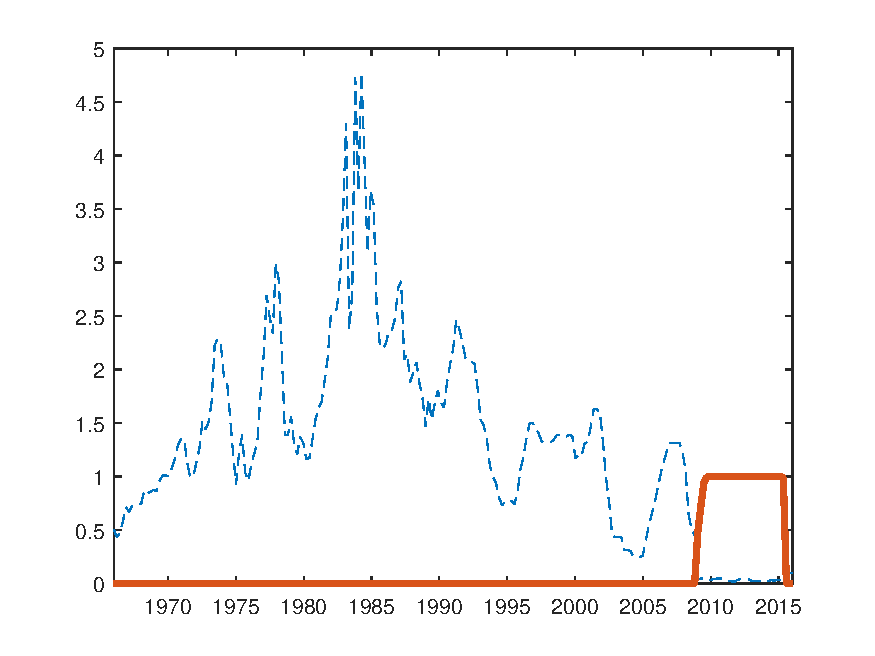
\includegraphics[scale=0.6]{NKPC_ree_init_AR1_regime.pdf}
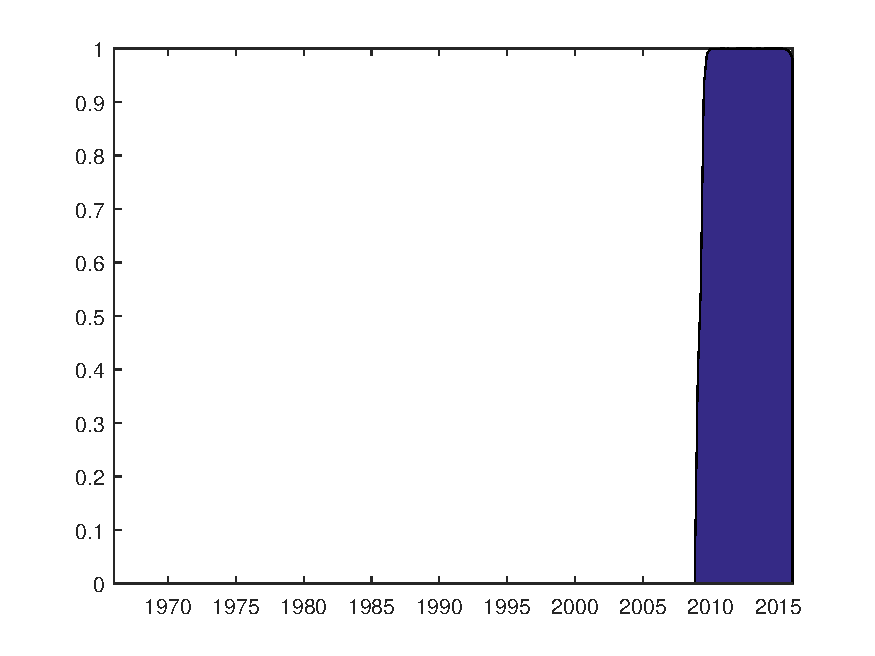
\includegraphics[scale=0.6]{NKPC_ree_init_AR1_regimeProb.pdf}\\

\textbf{Expectation coefficients. Intercepts on the left, first-order autocorrelations on the right.}\\

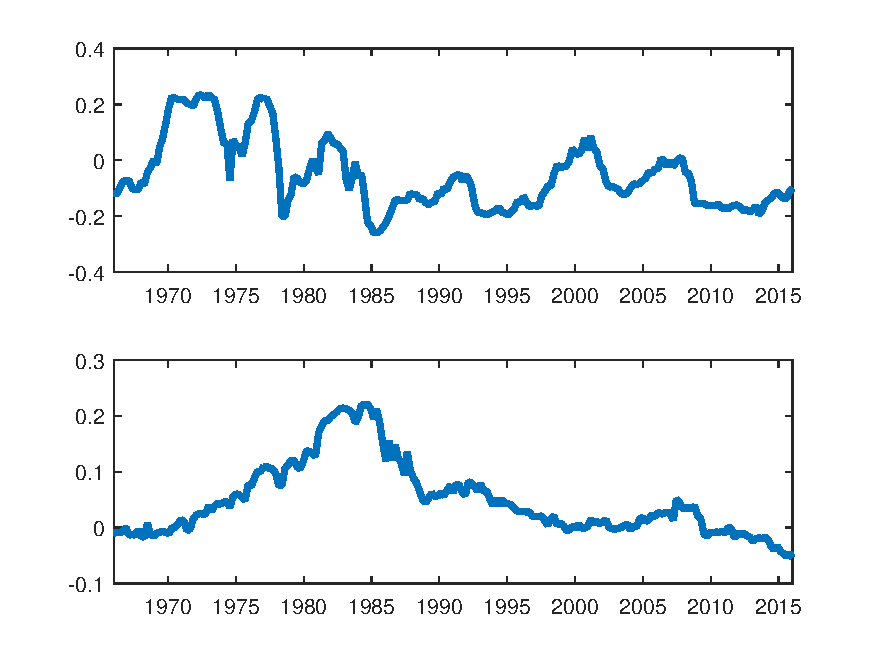
\includegraphics[scale=0.6]{NKPC_ree_init_AR1_alphas.pdf}
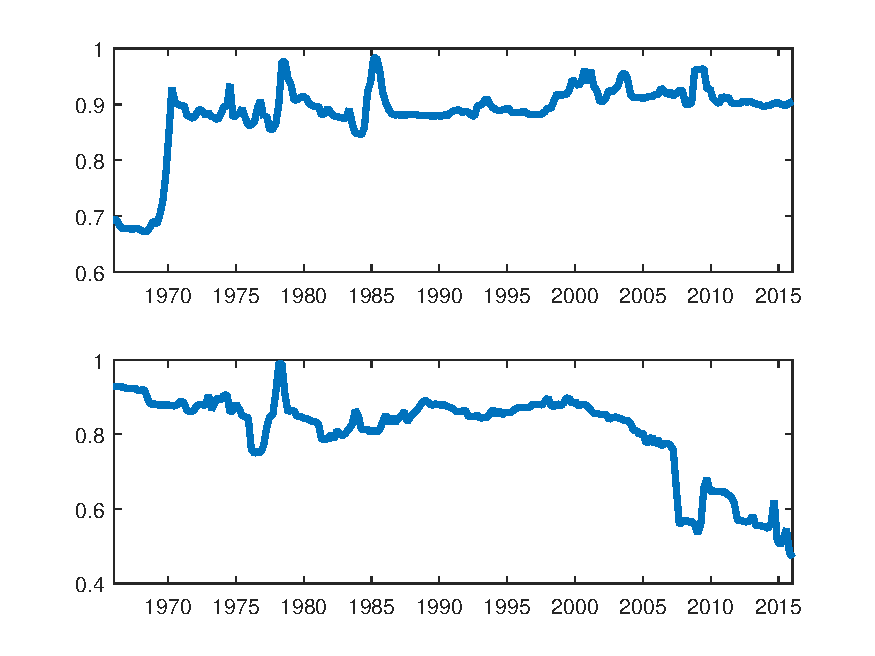
\includegraphics[scale=0.6]{NKPC_ree_init_AR1_betas.pdf}

\end{figure}

\newpage

\begin{figure}[H]
\caption{\large{\textbf{VAR(1)}}}
\vspace{5 mm}

\textbf{Interest rates and regime probability:} \\

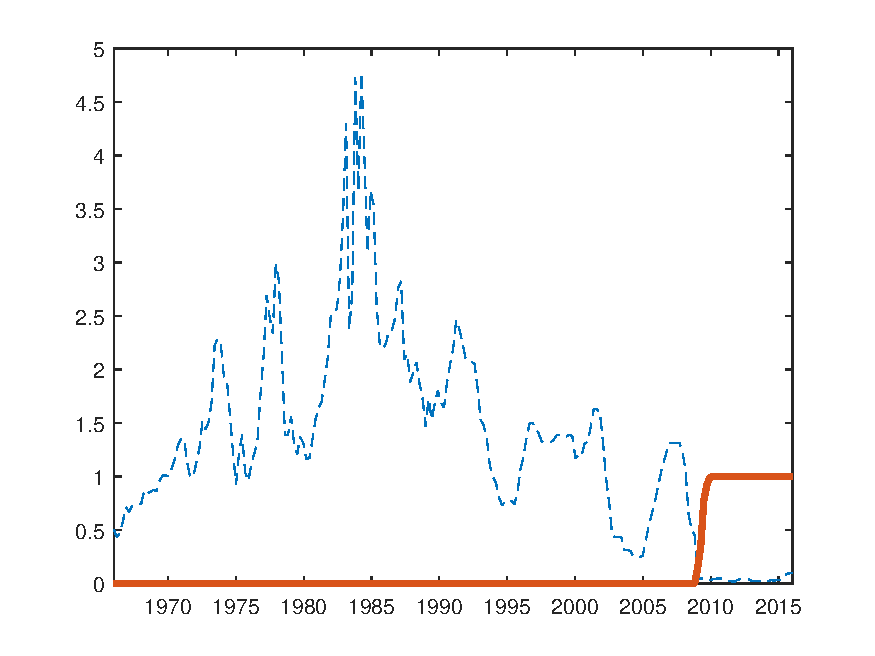
\includegraphics[scale=0.6]{NKPC_ree_init_VAR1_regime.pdf}
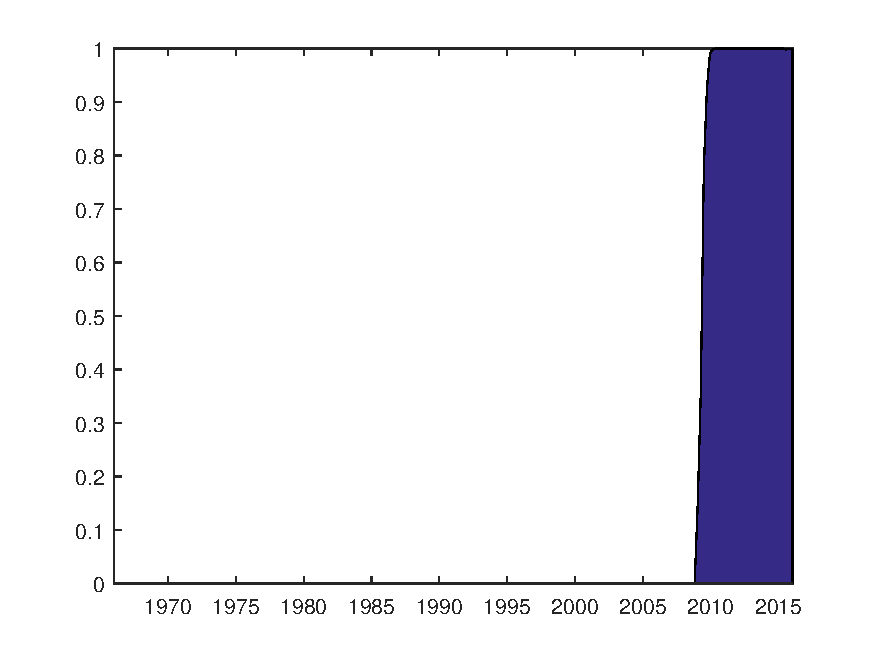
\includegraphics[scale=0.6]{NKPC_ree_init_VAR1_regimeProb.pdf}\\

\textbf{Expectation coefficient. Intercepts on the left, first-order autocorrelations on the right.}\\

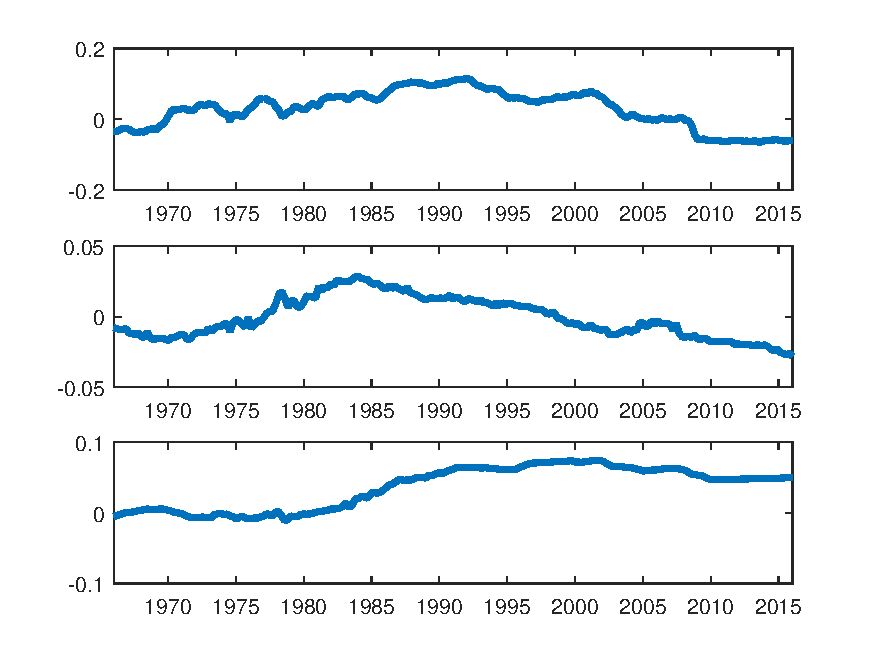
\includegraphics[scale=0.6]{NKPC_ree_init_VAR1_alphas.pdf}
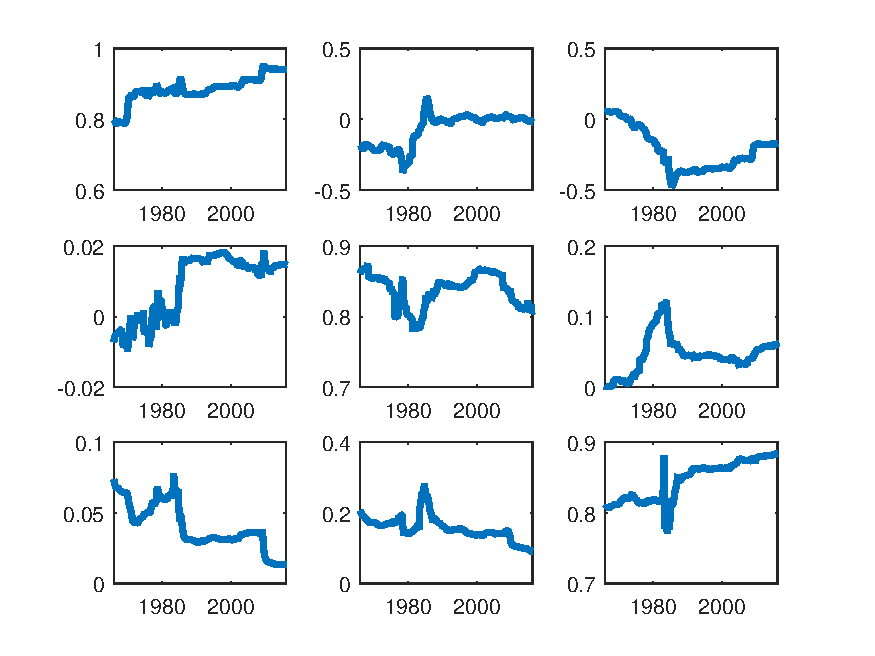
\includegraphics[scale=0.6]{NKPC_ree_init_VAR1_betas.pdf}


\end{figure}

\newpage

\begin{figure}[H]
\caption{\large{\textbf{MSV}}}
\vspace{5 mm}

\textbf{Interest rates and regime probability:} \\

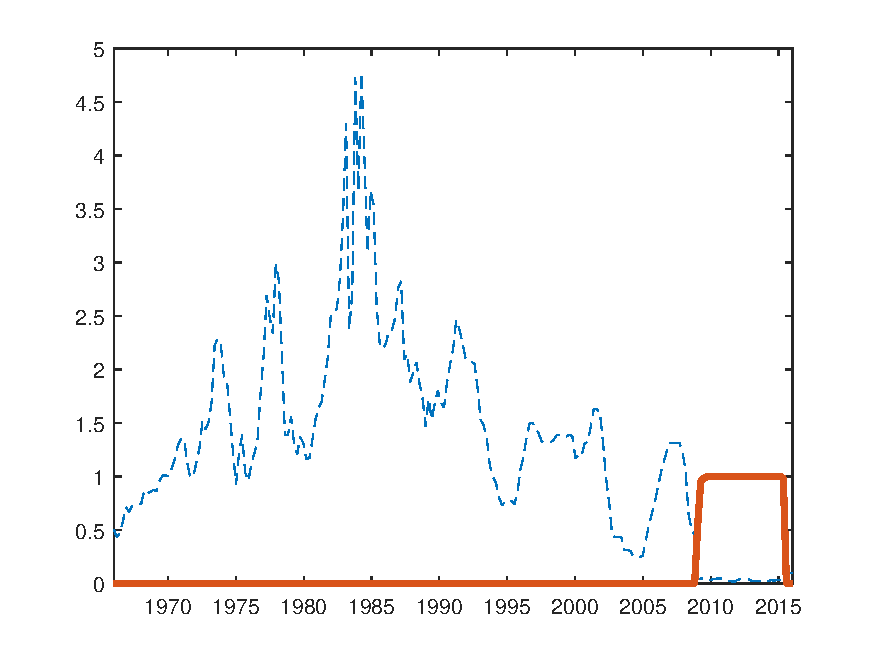
\includegraphics[scale=0.6]{NKPC_ree_init_MSV_regime.pdf}
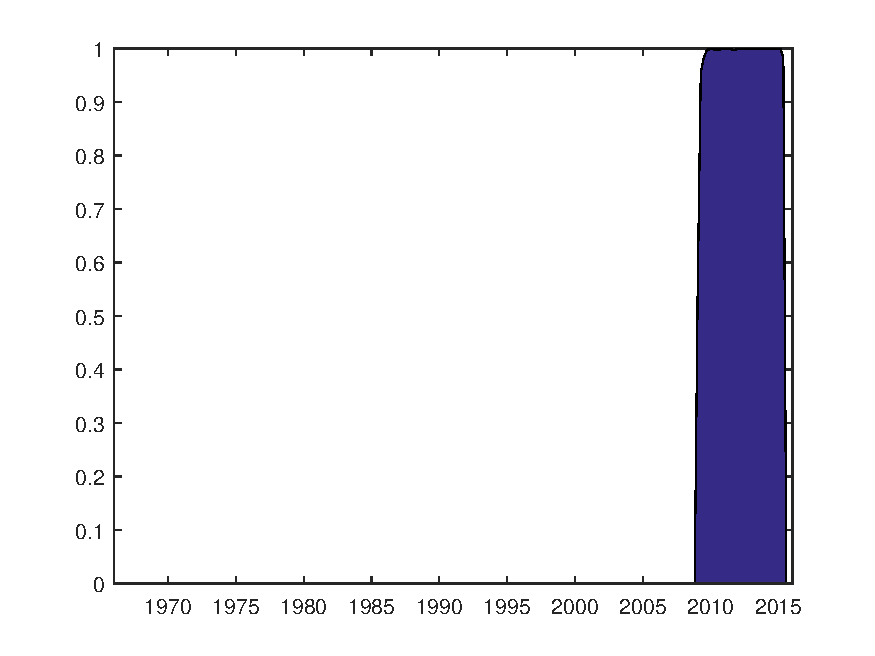
\includegraphics[scale=0.6]{NKPC_ree_init_MSV_regimeProb.pdf}\\

\textbf{Expectation coefficients. Intercepts on the left, first-order autocorrelations on the right}\\

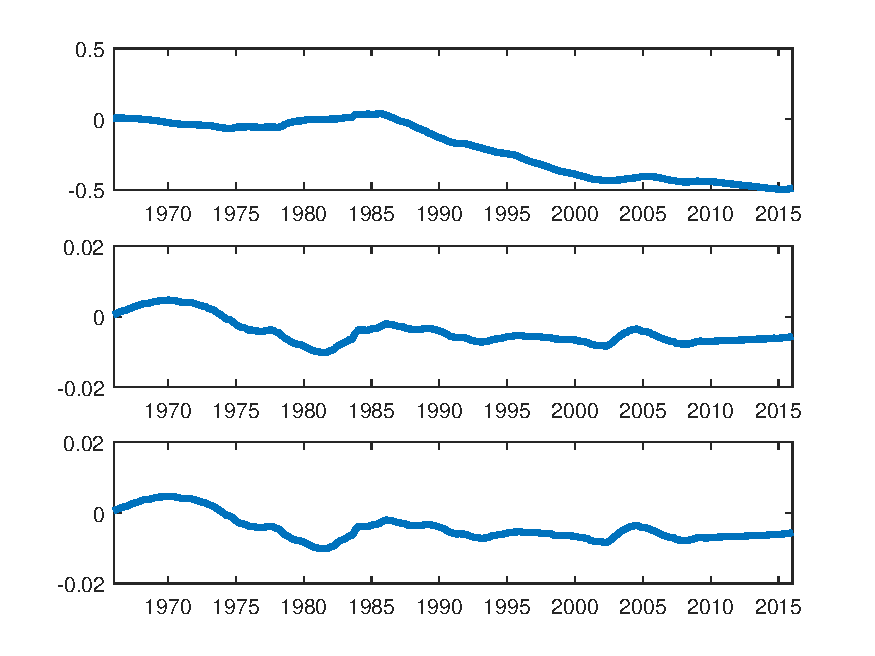
\includegraphics[scale=0.6]{NKPC_ree_init_MSV_alphas.pdf}
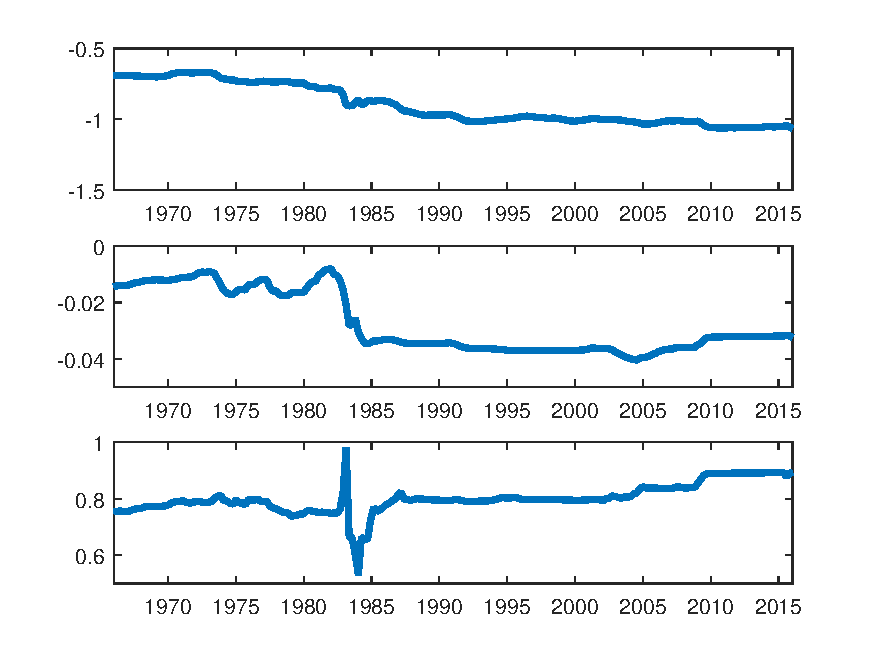
\includegraphics[scale=0.6]{NKPC_ree_init_MSV_betas.pdf}\\

\textbf{Shock coefficients:}\\

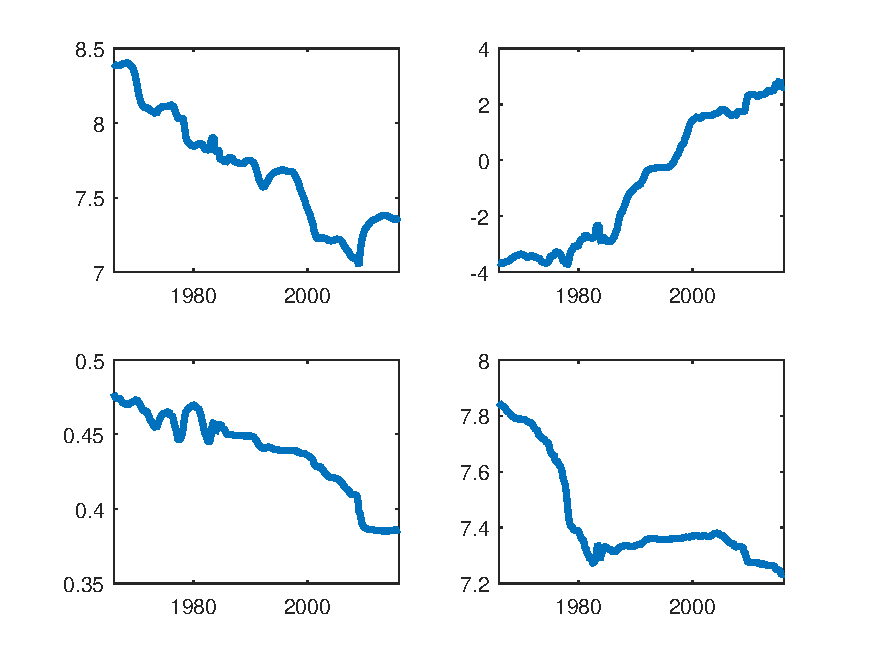
\includegraphics[scale=0.6]{NKPC_ree_init_MSV_shockCoef.pdf}\\


\end{figure}


\begin{figure}[H]
\caption{\large{\textbf{MSV-REE }}}
\vspace{5 mm}

\textbf{Interest rates and regime probability:} \\

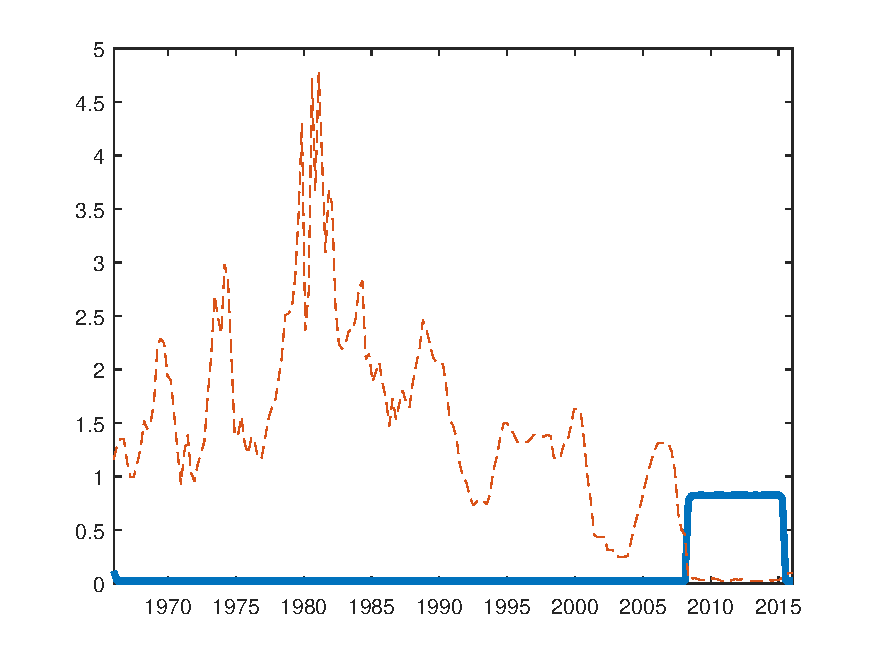
\includegraphics[scale=0.6]{NKPC_sigmaPoint_regime.pdf}
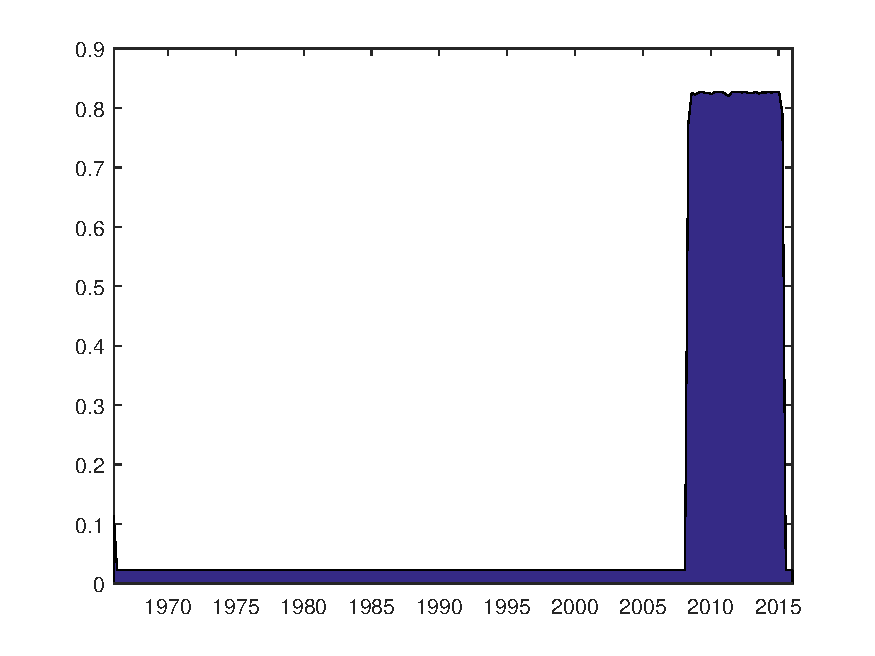
\includegraphics[scale=0.6]{NKPC_sigmaPoint_regimeProb.pdf}\\




\end{figure}

\newpage

\section*{Estimating the Baseline NKPC: Optimized initial beliefs} 

\begin{table}[H]
\begin{tabular}{l||lll||l|l|l|ll}
Parameter & Prior &  &  & Posterior &  &  &  &  \\
\hline
\hline
 &  &  &  & AR(1) & VAR(1) & MSV & REE-MS & REE \\
\hline
\hline
 & Dist & Mean & St. Dev & Mode & Mode & Mode & Mode & Mode  \\
$\bar{y}$ & Normal & 0 & 0.25 & -0.15 & 0.05 & -0.35 & -0.17 & 0.24 \\
$\bar{\pi}$ & Gamma & 0.62 & 0.25 & 0.49 & 0.96 & 0.69 & 0.39 & 0.17 \\
$\bar{r_1}$ & Gamma & 1 & 0.25 & 1.03 & 1.34 & 0.88 & 0.68 & 1.11 \\
$\kappa$ & Beta & 0.3 & 0.15 & 0.03 & 0.03 & 0.038 & 0.004 & 0.006 \\
$\tau$ & Gamma & 2 & 0.5 & 2.52 & 3.11 & 2.6 & 4.73 & 4.57 \\
$\phi_{\pi}$ & Gamma & 1.5 & 0.25 & 1.25 & 1.32 & 1.55 & 1.56 & 1.42 \\
$\phi_y$ & Gamma & 0.5 & 0.25 & 0.59 & 0.36 & 0.37 & 0.27 & 0.27 \\
$\rho_y$ & Beta & 0.5 & 0.2 & 0.3 & 0.39 & 0.91 & 0.92 & 0.93 \\
$\rho_{\pi}$ & Beta & 0.5 & 0.2 & 0.05 & 0.05 & 0.81 & 0.92 & 0.89 \\
$\rho_r$ & Beta & 0.5 & 0.2 & 0.95 & 0.97 & 0.89 & 0.8 & 0.8 \\
$\eta_y$ & Inv. Gamma & 0.1 & 2 & 0.76 & 0.75 & 0.09 & 0.1 & 0.1 \\
$\eta_{\pi}$ & Inv. Gamma & 0.1 & 2 & 0.26 & 0.26 & 0.04 & 0.03 & 0.04 \\
$\eta_{r_1}$ & Inv. Gamma & 0.1 & 2 & 0.32 & 0.33 & 0.32 & 0.32 & 0.3 \\
$\bar{r_2}$ & Normal & 0 & 0.25 & 0.04 & 0.04 & 0.03 & 0.03 & - \\
$\eta_{r_2}$ & Inv. Gamma & 0.01 & 0.2 & 0.02 & 0.02 & 0.01 & 0.01 & - \\
$1-p_{11}$ & Beta & 0.1 & 0.05 & 0.02 & 0.02 & 0.02 & 0.02 & - \\
$1-p_{22}$ & Beta & 0.3 & 0.1 & 0.1 & 0.1 & 0.13 & 0.17 & - \\
$gain$ & Gamma & 0.035 & 0.015 & 0.04 & 0.0382 & 0.0085 & - & - \\
\hline
\hline
Laplace &  &  &  & -294.123 & -308.92 & -282.62 & -317.02 & -368.49
\end{tabular}
\end{table}

\begin{figure}[H]
\caption{\large{\textbf{AR(1)}}}
\vspace{5 mm}

\textbf{Interest rates and regime probability:} \\

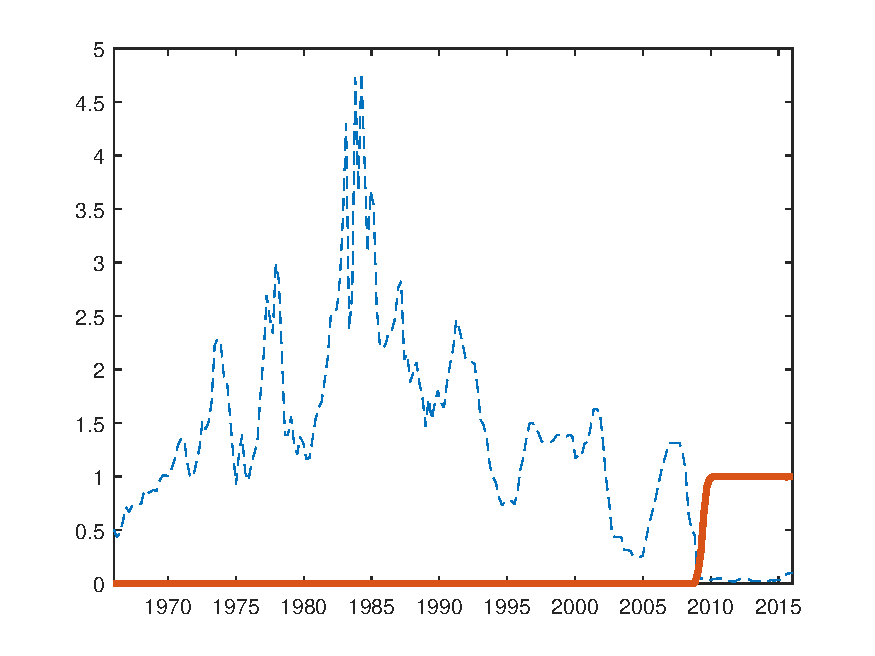
\includegraphics[scale=0.6]{NKPC_optim_init_AR1_regime.pdf}
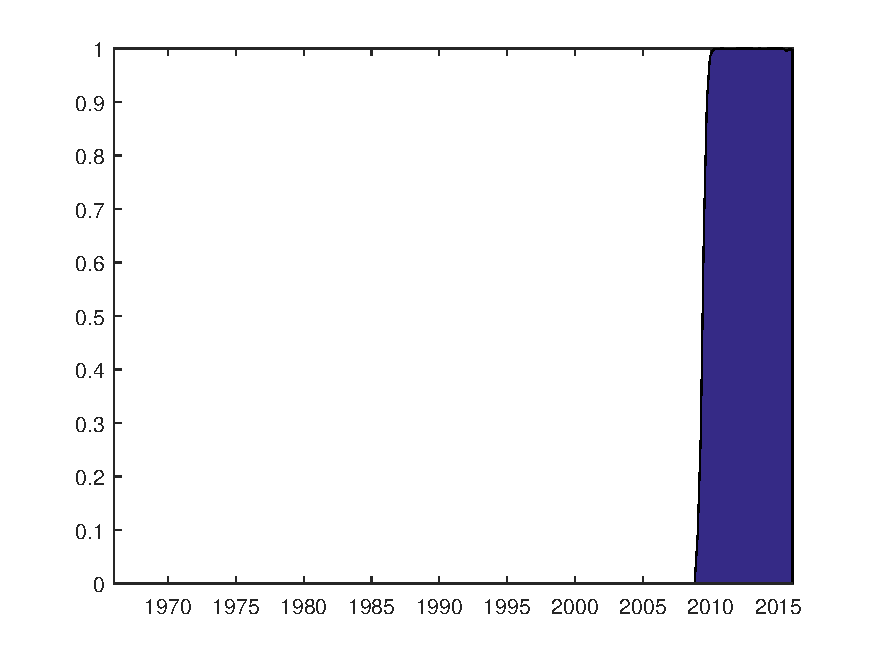
\includegraphics[scale=0.6]{NKPC_optim_init_AR1_regimeProb.pdf}\\

\textbf{Expectation coefficients. Intercepts on the left, first-order autocorrelations on the right.}\\

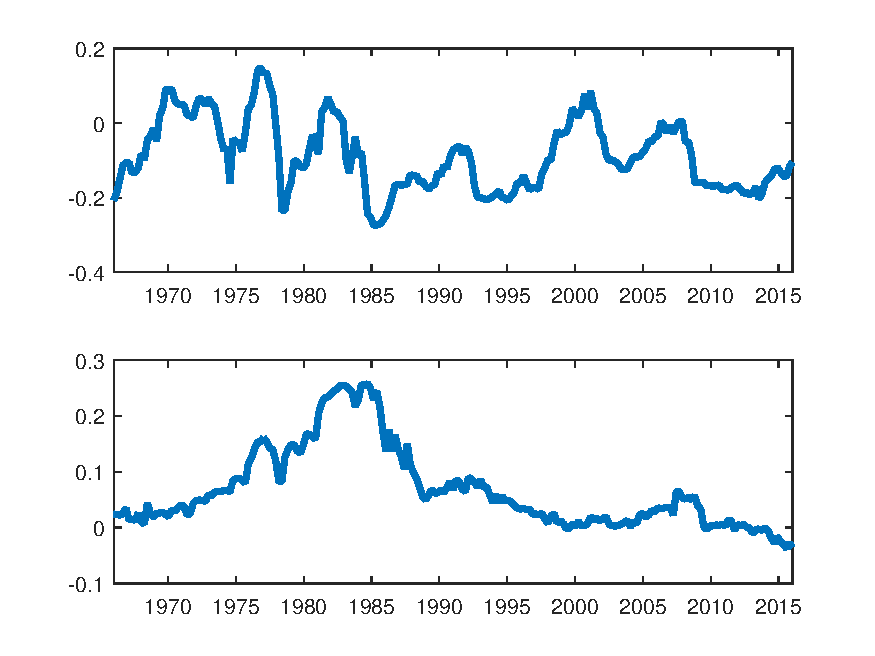
\includegraphics[scale=0.6]{NKPC_optim_init_AR1_alphas.pdf}
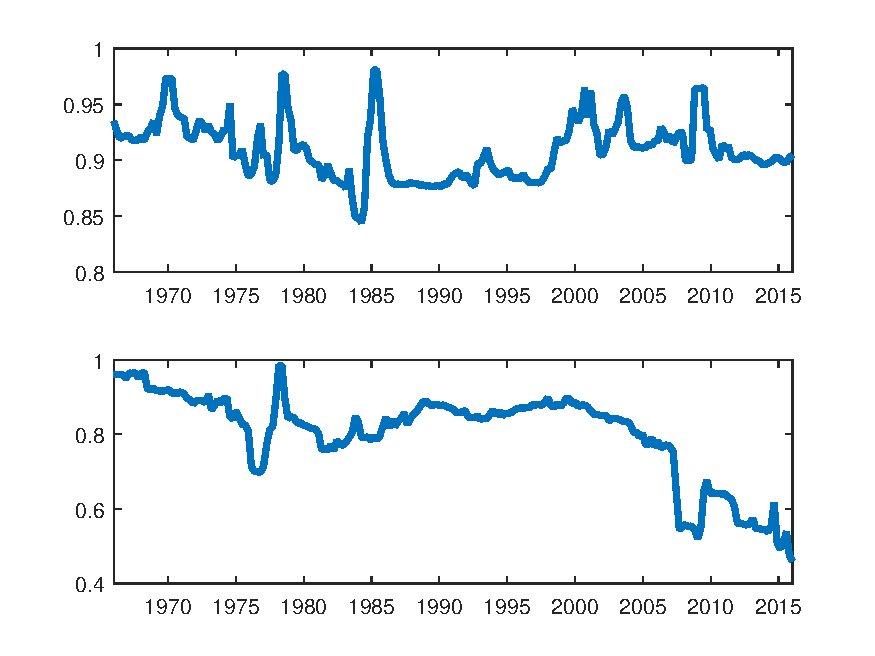
\includegraphics[scale=0.6]{NKPC_optim_init_AR1_betas.pdf}


\end{figure}

\newpage

\begin{figure}[H]
\caption{\large{\textbf{VAR(1)}}}
\vspace{5 mm}

\textbf{Interest rates and regime probability:} \\

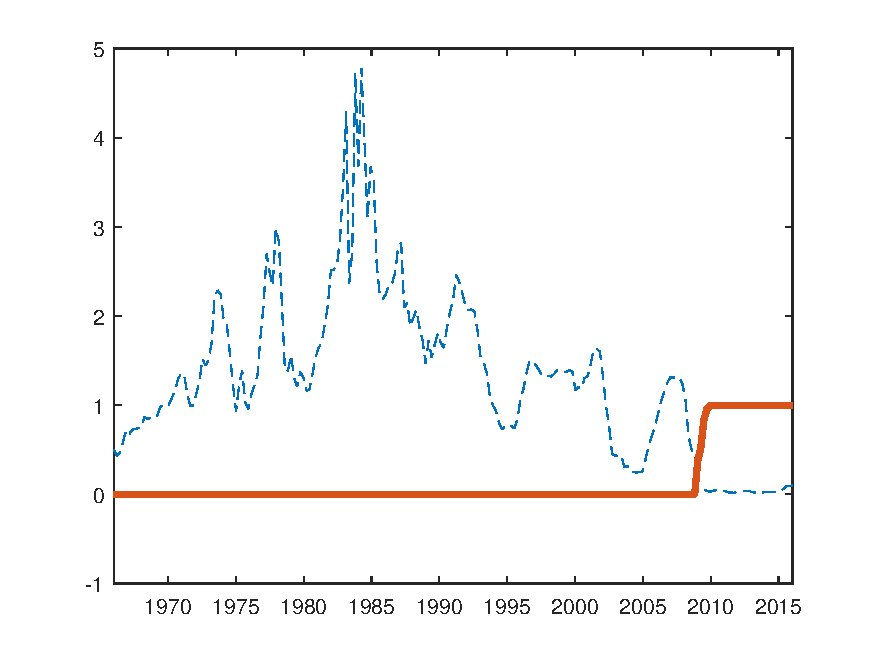
\includegraphics[scale=0.6]{NKPC_optim_init_VAR1_regime.pdf}
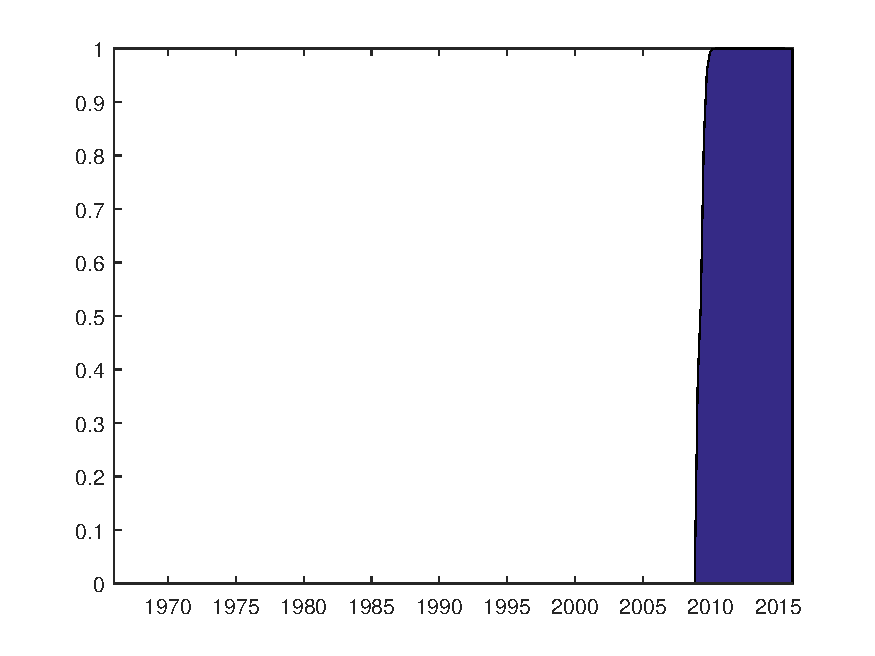
\includegraphics[scale=0.6]{NKPC_optim_init_VAR1_regimeProb.pdf}\\

\textbf{Expectation coefficient. Intercepts on the left, first-order autocorrelations on the right.}\\

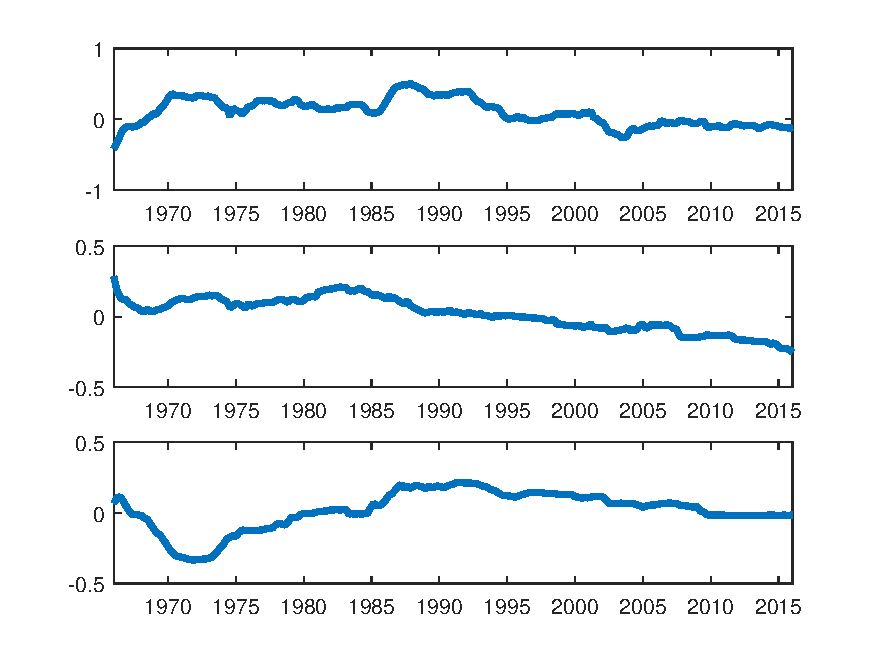
\includegraphics[scale=0.6]{NKPC_optim_init_VAR1_alphas.pdf}
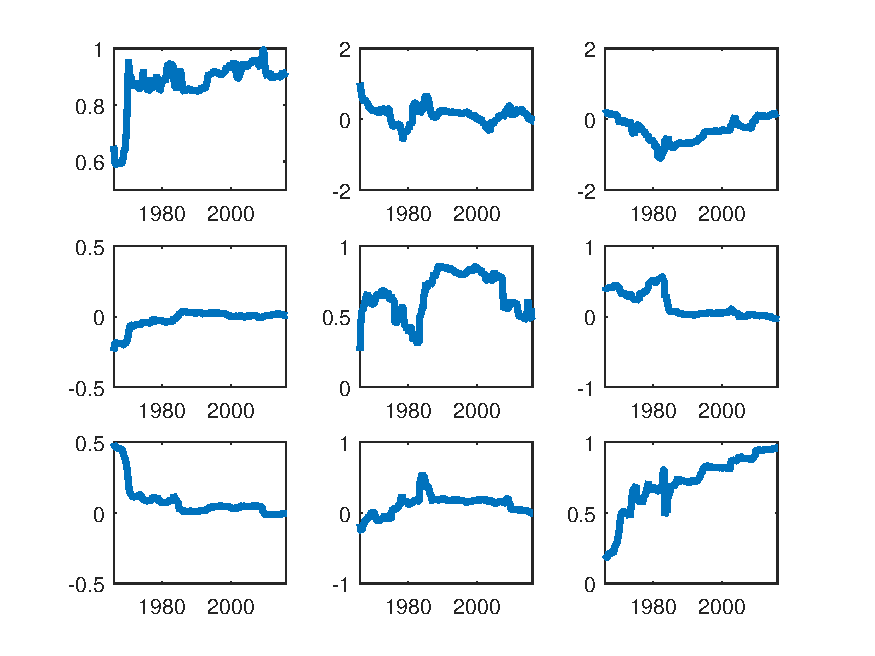
\includegraphics[scale=0.6]{NKPC_optim_init_VAR1_betas.pdf}


\end{figure}

\newpage

\begin{figure}[H]
\caption{\large{\textbf{MSV}}}
\vspace{5 mm}

\textbf{Interest rates and regime probability:} \\

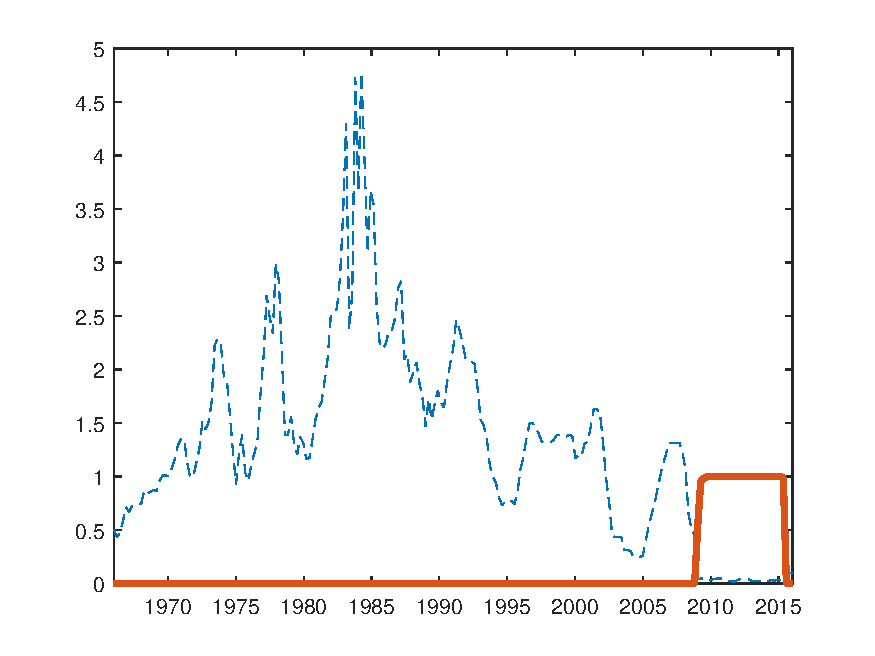
\includegraphics[scale=0.6]{NKPC_optim_init_MSV_regime.pdf}
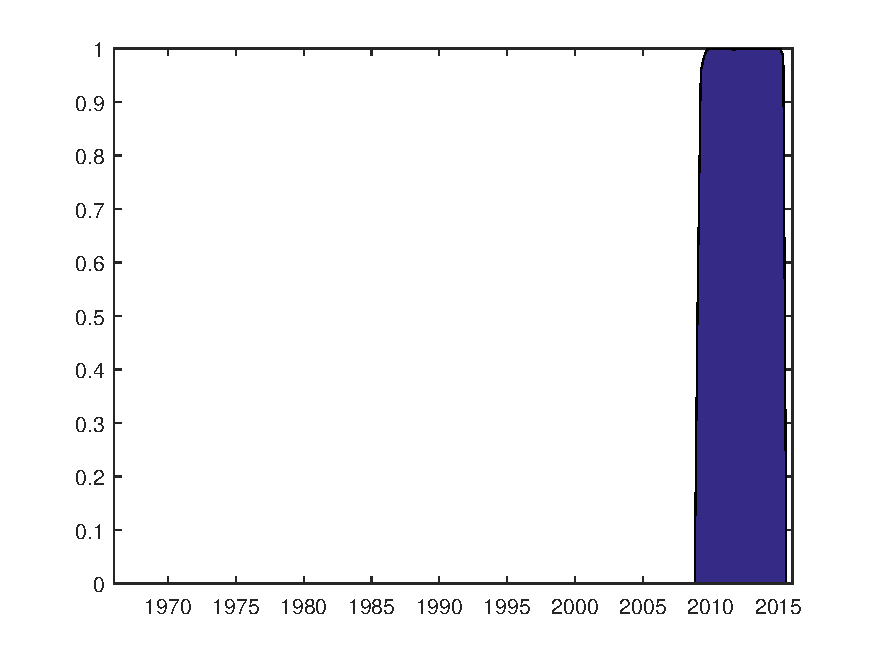
\includegraphics[scale=0.6]{NKPC_optim_init_MSV_regimeProb.pdf}\\

\textbf{Expectation coefficients. Intercepts on the left, first-order autocorrelations on the right}\\

\includegraphics[scale=0.6]{NKPC_optim_init_MSV_alphas.pdf}
\includegraphics[scale=0.6]{NKPC_optim_init_MSV_betas.pdf}\\

\textbf{Shock coefficients:}\\

\includegraphics[scale=0.6]{NKPC_optim_init_MSV_shockCoef.pdf}\\


\end{figure}


\section*{Estimating the Baseline NKPC: Filter-based initial beliefs} 



\begin{table}[H]
\begin{tabular}{l||lll||l|l|l|ll}
Parameter & Prior &  &  & Posterior &  &  &  &  \\
\hline
\hline
 &  &  &  & AR(1) & VAR(1) & MSV & REE-MS & REE \\
\hline
\hline
 & Dist & Mean & St. Dev & Mode & Mode & Mode & Mode &  \\
$\bar{y}$ & Normal & 0 & 0.25 & -0.16 & -0.01 & -0.26 & -0.17 & 0.24 \\
$\bar{\pi}$ & Gamma & 0.62 & 0.25 & 0.47 & 0.46 & 0.54 & 0.39 & 0.17 \\
$\bar{r_1}$ & Gamma & 1 & 0.25 & 0.99 & 1.03 & 0.86 & 0.68 & 1.11 \\
$\kappa$ & Beta & 0.3 & 0.15 & 0.03 & 0.0081 & 0.006 & 0.004 & 0.006 \\
$\tau$ & Gamma & 2 & 0.5 & 2.51 & 2.92 & 2.79 & 4.73 & 4.57 \\
$\phi_{\pi}$ & Gamma & 1.5 & 0.25 & 1.25 & 1.26 & 1.52 & 1.56 & 1.42 \\
$\phi_y$ & Gamma & 0.5 & 0.25 & 0.59 & 0.56 & 0.33 & 0.27 & 0.27 \\
$\rho_y$ & Beta & 0.5 & 0.2 & 0.3 & 0.52 & 0.92 & 0.92 & 0.93 \\
$\rho_{\pi}$ & Beta & 0.5 & 0.2 & 0.05 & 0.09 & 0.9 & 0.92 & 0.89 \\
$\rho_r$ & Beta & 0.5 & 0.2 & 0.95 & 0.96 & 0.87 & 0.8 & 0.8 \\
$\eta_y$ & Inv. Gamma & 0.1 & 2 & 0.76 & 0.74 & 0.12 & 0.1 & 0.1 \\
$\eta_{\pi}$ & Inv. Gamma & 0.1 & 2 & 0.26 & 0.27 & 0.04 & 0.03 & 0.04 \\
$\eta_{r_1}$ & Inv. Gamma & 0.1 & 2 & 0.32 & 0.32 & 0.32 & 0.32 & 0.3 \\
$\bar{r_2}$ & Normal & 0 & 0.25 & 0.04 & 0.04 & 0.03 & 0.03 & - \\
$\eta_{r_2}$ & Inv. Gamma & 0.01 & 0.2 & 0.02 & 0.02 & 0.01 & 0.01 & - \\
$1-p_{11}$ & Beta & 0.1 & 0.05 & 0.02 & 0.02 & 0.02 & 0.02 & - \\
$1-p_{22}$ & Beta & 0.3 & 0.1 & 0.1 & 0.1 & 0.13 & 0.17 & - \\
$gain$ & Gamma & 0.035 & 0.015 & 0.0421 & 0.0064 & 0.0075 & - & - \\
 &  &  &  &  &  &  &  &  \\
Laplace &  &  &  & -294.24 & -307.34 & -290 & -317.02 & -368.49
\end{tabular}
\end{table}

\begin{figure}[H]
\caption{\large{\textbf{AR(1)}}}
\vspace{5 mm}

\textbf{Interest rates and regime probability:} \\

\includegraphics[scale=0.6]{NKPC_filter_init_AR1_regime.pdf}
\includegraphics[scale=0.6]{NKPC_filter_init_AR1_regimeProb.pdf}\\

\textbf{Expectation coefficients. Intercepts on the left, first-order autocorrelations on the right.}\\

\includegraphics[scale=0.6]{NKPC_filter_init_AR1_alphas.pdf}
\includegraphics[scale=0.6]{NKPC_filter_init_AR1_betas.pdf}


\end{figure}

\newpage

\begin{figure}[H]
\caption{\large{\textbf{VAR(1)}}}
\vspace{5 mm}

\textbf{Interest rates and regime probability:} \\

\includegraphics[scale=0.6]{NKPC_filter_init_VAR1_regime.pdf}
\includegraphics[scale=0.6]{NKPC_filter_init_VAR1_regimeProb.pdf}\\

\textbf{Expectation coefficient. Intercepts on the left, first-order autocorrelations on the right.}\\

\includegraphics[scale=0.6]{NKPC_filter_init_VAR1_alphas.pdf}
\includegraphics[scale=0.6]{NKPC_filter_init_VAR1_betas.pdf}


\end{figure}

\newpage

\begin{figure}[H]
\caption{\large{\textbf{MSV}}}
\vspace{5 mm}

\textbf{Interest rates and regime probability:} \\

\includegraphics[scale=0.6]{NKPC_filter_init_MSV_regime.pdf}
\includegraphics[scale=0.6]{NKPC_filter_init_MSV_regimeProb.pdf}\\

\textbf{Expectation coefficients. Intercepts on the left, first-order autocorrelations on the right}\\

\includegraphics[scale=0.6]{NKPC_filter_init_MSV_alphas.pdf}
\includegraphics[scale=0.6]{NKPC_filter_init_MSV_betas.pdf}\\

\textbf{Shock coefficients:}\\

\includegraphics[scale=0.6]{NKPC_filter_init_MSV_shockCoef.pdf}\\


\end{figure}


\section*{Impulse Responses (using the REE-based initial beliefs setup)}

\begin{figure}[H]
\caption{Impulse responses of time-varying PLMs are based on an arbitrary period.}
\textbf{AR(1) and VAR(1) beliefs:}\\
\includegraphics[scale=0.6]{NKPC_ree_init_AR1_IR.pdf}
\includegraphics[scale=0.6]{NKPC_ree_init_VAR_IR.pdf}\\

\textbf{MS and standard REE benchmarks: }\\

\includegraphics[scale=0.6]{NKPC_ree_init_REE_MS_IR.pdf}
\includegraphics[scale=0.6]{NKPC_ree_init_REE_IR.pdf}\\

\textbf{MSV beliefs: }\\

\includegraphics[scale=0.6]{NKPC_ree_init_MSV_IR.pdf}\\
\end{figure}

\newpage

\begin{figure}[H]
\caption{Time-varying impulse responses, final 50 periods of the estimation sample.}

\textbf{AR(1)}: \\
\includegraphics[scale=1]{NKPC_ree_init_AR1_IR_timeVarying.pdf}\\
\end{figure}

\begin{figure}[H]
\caption{Time-varying impulse responses, final 50 periods of the estimation sample.}

\textbf{VAR(1)}: \\
\includegraphics[scale=1]{NKPC_ree_init_VAR_IR_timeVarying.pdf}\\
\end{figure}

\begin{figure}[H]
\caption{Time-varying impulse responses, final 50 periods of the estimation sample.}

\textbf{MSV}: \\
\includegraphics[scale=1]{NKPC_ree_init_MSV_IR_timeVarying.pdf}\\
\end{figure}


\begin{comment}
this part became redundant now...
\newpage
\subsection*{General Setup} 

DGP: $ X_t = A(s_t) + B(s_t) E_t X_{t+1} + C(s_t) X_{t-1} + D(s_t) \epsilon_t$. \\

PLM: $ X_t = a+ c X_{t-1} + d \eta_t  \Rightarrow E_t X_{t+1} = a + c E_t X_t = a + c(a+ c X_{t-1})=  (a + ca) + c^2 X_{t-1} $. \\

Implied ALM: \\

$ X_t = A(s_t) + B(s_t) ( (a+ca) + c^2 X_{t-1}) + C(s_t) X_{t-1} + D(s_t) \epsilon_t $. \\

$ \rightarrow X_t = A(s_t) + B(s_t) (a+ca) + (B(s_t)c^2 + C(s_t))X_{t-1} + D(s_t) \epsilon_t $. \\

Consistency conditions: \\

$a = E(X_t) $ (Vector of unconditional means)\\

$ c= \frac{E[X_t X_{t-1}']}{E[X_t X_t']} $ (Matrix of unconditional auto- and cross-correlations.) \\

Transition matrix Q same as before , with $ \pi = [ \frac{1-p_{22}}{2-p_{11}- p_{22}}, \frac{1-p_{11}}{2-p_{11}-p_{22}}] $.\\

(i)  From implied ALM, we have \\

$ E[X_t] = \sum_i \pi_i A_i + \sum_i \pi_i B_i(a+ca) + (\sum_i \pi_i B_i c^2 + \sum_i pi_i C_i) E[X_{t-1}]. $\\

Using $ E[X_t ] = E[X_{t-1}]=a : $ \\

$a = \sum_i \pi_i A_i + \sum_i \pi_i B_i (a+ca) + (\sum_i \pi_i B_i c^2 + \sum_i \pi_i c_i ) a $. \\

$ a = (I - \sum_i \pi_i B_i - c \sum_i \pi_i B_i  - \sum_i \pi_i C_i - \sum_i \pi_i B_i c^2 )^{(-1)} \sum_i \pi_i A_i $. \\

Consider the simple case where $ A(s_t) = 0 \forall s_t $. Then we have \\

$$ X_t = B(s_t) (a+ca) + (B(s_t) c^2 + C(s_t))X_{t-1} + D(s_t) \epsilon_t.$$\\

Denote $ E[X_t X_t']= \Gamma_0 $ and $E[X_t X_{t-1}']=\Gamma_1 $. \\

The first-two Yule-Walker equations yield: \\

(i) $\Gamma_1 = E[ B(s_t) c^2 + C(s_t)] \Gamma_0 $. \\

$ \Gamma_1 = \sum_i \pi_i B_i c^2 + \sum_i \pi_i C_i = c^2 \sum_i \pi_i B_i + \sum_i \pi_i C_i $. \\

Denoting $ c^2 \sum_i \pi_i B_i + \sum_i \pi_i = M(c) $, we get \\

$$ \Gamma_1 = M(c) \Gamma_0 $$. \\

(ii) $Var(X_t) = M(c) Var(X_{t-1}) M(c)' + (\sum_i \pi_i D_i ) \Sigma_{\epsilon} (\sum_i \pi_i D_i)' $.

Denoting $\sum_i \pi_i D_i  = \tilde{D} $, we get \\

$$ \vec(\Gamma_0) = (I-M(c) \otimes M(c) )^{(-1)} (\tilde{D} \otimes \tilde{D}) vec(\Sigma_{\epsilon}). $$

Hence 

$$ c(i,j) =\frac{ vec(\Gamma_1)_{(j-1)N+j}}{ vec(\Gamma_0)_{(j-1)N+j}} $$

Collecting everything, c solves the following:\\

$$
\begin{cases}
c= \Gamma_1 \oslash \Gamma_0 \\
\Gamma_1 = M(c) \Gamma_0 \\
 \vec(\Gamma_0) = (I-M(c) \otimes M(c) )^{(-1)} (\tilde{D} \otimes \tilde{D}) vec(\Sigma_{\epsilon})\\
\tilde{D} = \sum_i \pi_i D_i   \\
 M(c) = c^2 \sum_i \pi_i B_i + \sum_i \pi_i \\

\end{cases}
$$

The T-map is given by : \\
$$
\begin{pmatrix} a \\ c \end{pmatrix} \Rightarrow \begin{pmatrix} A(s_t) + B(s_t) (a+ca) \\ B(s_t) c^2 + C(s_t) \end{pmatrix}$$


\newpage

\end{comment}


\end{document}

